\documentclass[11pt, french]{book}
\usepackage{natbib}
\usepackage[french]{babel}
\selectlanguage{french}
\usepackage[T1]{fontenc}
\usepackage[utf8]{inputenc}
\usepackage{geometry}
\usepackage{array}
\usepackage{mathpazo}
\usepackage{microtype}
\usepackage[margin=17pt, font=small, labelfont={bf,sf}]{caption}
\geometry{
    verbose,
    tmargin=3cm,
    bmargin=3cm,
    lmargin=1.8cm,
    rmargin=1.8cm,
    headheight=3cm,
    headsep=0.5cm,
    footskip=0.8cm
}
\pagestyle{empty}
\setcounter{secnumdepth}{3}
\setcounter{tocdepth}{3}
\usepackage{verbatim}
\usepackage{multirow}
\usepackage{multicol}
\usepackage{setspace}
\setstretch{1.1}
\usepackage{float}
\usepackage{url}
\usepackage{lipsum}
\usepackage{enumitem}
\setlist[itemize]{label=$\bullet$, nosep} % Setting default parameters for itemize env.

\usepackage{amsmath}
\usepackage{eurosym}
\usepackage{graphicx}
\usepackage{adjustbox}
\usepackage{nomencl}
\usepackage{listings}
\providecommand{\printnomenclature}{\printglossary}
\providecommand{\makenomenclature}{\makeglossary}
\makenomenclature
\makeatletter

\usepackage{wrapfig}


\providecommand{\tabularnewline}{\\}
\usepackage{tabularx}
\usepackage{babel}
\usepackage{fancyhdr}
\usepackage{color}
\usepackage[usenames, dvipsnames, svgnames, table]{xcolor}
\usepackage[french]{minitoc}
\usepackage{alertmessage}
\usepackage[
    breaklinks=true,
    unicode=true,
    colorlinks=true,
    linkcolor=tablemat,
    citecolor=citation,
    urlcolor=Blue
]{hyperref}
\hypersetup{final}
\usepackage{cleveref}
\crefname{figure}{Fig.}{Fig.}
\crefname{table}{Tab.}{Tab.}
\crefname{section}{Sec.}{Sec.}
\crefname{equation}{Eq.}{Eq.}
\usepackage[useregional]{datetime2}
\DTMsetdatestyle{ddmmyyyy}
\DTMsetup{datesep=/}
\usepackage{sectsty}
\allsectionsfont{\sffamily}
\newcommand{\script}[1]{{\ttfamily\bfseries {#1}}}

\definecolor{tablemat}{rgb}{0.18,0.32,0.32}
\definecolor{citation}{rgb}{0,0,0.45}
\definecolor{darkWhite}{rgb}{0.98,0.98,0.98}
\definecolor{darkGreen}{rgb}{0,0.5,0}
\pagestyle{fancy}
\renewcommand{\headrulewidth}{1pt}
\fancyhead[LE]{\thepage}
\fancyhead[RE]{\textbf{\leftmark}}
\fancyhead[RO]{\thepage}
\fancyhead[LO]{\textbf{\rightmark}}
\fancyfoot[L,C,R]{}

% Fills pages starting from the top !
\raggedbottom

% Settings for COMM/code/command excerpts
\lstset{aboveskip=6mm,belowskip=-3.mm,backgroundcolor=
\color{darkWhite}
, basicstyle=\ttfamily\footnotesize,breakatwhitespace=false, breaklines=true,captionpos=b,commentstyle=
\color{blue}
,deletekeywords={...},escapeinside={\%*}{*)},extendedchars=true, framexleftmargin=0pt,
framextopmargin=2pt,framexbottommargin=2pt,frame=tb, keepspaces=true,
keywordstyle=
\color{blue}
, language=C,morekeywords={*,...}, numbers=left,numbersep=3pt,numberstyle=\tiny
\color{black}
,rulecolor=
\color{black}
,showspaces=false,showstringspaces=false,showtabs=false,stepnumber=1,
stringstyle=
\color{gray}
, tabsize=3, title=\lstname, morecomment=[l][
\color{blue}
]{!}}

\lstdefinelanguage{json}{
    basicstyle=\footnotesize\ttfamily,   % Police de base
    commentstyle=\color{olive},          % Style des commentaires
    keywordstyle=\color{blue},           % Style des mots-clés
    numberstyle=\tiny\color{gray},       % Style des numéros de ligne
    numbers=left,                        % Numérotation à gauche
    stringstyle=\color{purple},          % Style des chaînes de caractères
    breaklines=true,                     % Coupure automatique des lignes
    showstringspaces=false,              % Pas d'espaces visibles dans les chaînes
    tabsize=2,                           % Taille des tabulations
    frame=lines,                         % Encadrement du code
    captionpos=b,                        % Position de la légende en bas
    aboveskip=15pt,                      % Espace avant le listing
    belowskip=15pt,                      % Espace après le listing
    comment=[l]{//},                     % Commentaires ligne avec //
    morecomment=[s]{/*}{*/}              % Commentaires multi-lignes /* */
}

% Pour les notes de rédaction dans le document
\usepackage{todonotes}

\renewcommand{\lstlistingname}{Code}
\renewcommand{\lstlistlistingname}{Liste des codes}



% Alertmessage pkg command memo
% \alertinfo{Test.}
% \alertsuccess{Test.}
% \alertwarning{Test.}
% \alerterror{Test.}

% Pour des entêtes de chapitre
\usepackage[Bjornstrup]{fncychap}
\ChRuleWidth{0.2pt}
\ChNameVar{\Large\bfseries}
\ChNameUpperCase
\ChTitleVar{\bfseries\large\rm}
\addto\captionsfrench{\def\tablename{Tableau}}
\ChNumVar{\Large{\textbf{\color{white}{CHAPITRE}}} \fontsize{76}{80}\usefont{OT1}{pzc}{m}{n}\selectfont}
\ChTitleVar{\raggedright\LARGE\bfseries}
\newcommand{\colortitlechap}{\color[rgb]{1,1,1}} % color of the chapter title
\newcommand{\colornumberchap}{\color[rgb]{0.7,0.8,0.2}} % color of the chapter number
\newcommand{\colorbackchap}{\colorbox[rgb]{0.18,0.32,0.32}} % color of the background box (= tablemat color)

% Custom setup for chapter headers
\makeatletter
\renewcommand{\DOCH}{%
\settowidth{\py}{\CNoV\thechapter}
\addtolength{\py}{-10pt}%
\fboxsep=0pt%
\colorbackchap{\rule{0pt}{40pt}\parbox[b]{\textwidth}{\hfill}}%
\kern-\py\raise20pt%
\hbox{\colornumberchap\CNoV\thechapter}\\%
}

\renewcommand{\DOTI}[1]{%
\nointerlineskip\raggedright%
\fboxsep=\myhi%
\vskip-1ex%
\colorbackchap{\parbox[t]{\mylen}{\CTV\FmTi{\colortitlechap#1}}}\par\nobreak%
\vskip 40\p@%
}

\renewcommand{\DOTIS}[1]{%
\fboxsep=0pt%
\colorbackchap{\rule{0pt}{40pt}\parbox[b]{\textwidth}{\hfill}}\\%
\nointerlineskip\raggedright%
\fboxsep=\myhi%
\colorbackchap{\parbox[t]{\mylen}{\CTV\FmTi{\colortitlechap#1}}}\par\nobreak%
\vskip 40\p@%
}


\newcommand{\cwuserguide}{\footnote{Notice CaWaQS : \href{https://gitlab.com/cawaqs/cawaqs/-/raw/main/docs/CaWaQS_350_Documentation.pdf?ref_type=heads}{https://gitlab.com/cawaqs/cawaqs/-/raw/main/docs/CaWaQS_350_Documentation.pdf?ref_type=heads}}}
\makeatother

\usepackage{babel}
\makeatletter
\addto\extrasfrench{%
\providecommand{\og}{\leavevmode\flqq~}%
\providecommand{\fg}{\ifdim\lastskip>\z@\unskip\fi~\frqq}%
}

\makeatother
\def\eqdeclaration#1{, voir équation\nobreakspace(#1)}
\def\pagedeclaration#1{, page\nobreakspace#1}
\def\nomname{Liste des symboles}

% Format paysage
\usepackage{pdflscape}
\usepackage{subcaption}

\input{shortcuts}

\begin{document}
    \frontmatter
    \dominitoc%
    \begin{comment}
Début du bloc avec numérotation romaine
\end{comment}

    \include{couverture/couverture}

    \chapter*{Introduction}
\phantomsection
\addstarredchapter{\textbf{Introduction}}

\fancyhead[LE]{\thepage} 
\fancyhead[RE]{\textbf{Introduction}}
\fancyhead[RO]{\thepage} 
\fancyhead[LO]{\textbf{Introduction}}
\fancyfoot[C]{\thepage}

\setlength{\parindent}{0.35cm} 

% ====================================================

L'outil de visualisation \cwv~a été développé dans le but de visualiser, sous SIG, les sorties de modélisation de la plate-forme de modélisation \cws\cwversion. Cette extension fonctionne actuellement sous QGIS dans sa version \qgisversion.\\

\cwv~est structuré en divers outils et fonctionnalités aidant au processus de calibration d'une application \cawaqs~et facilitant la visualisation des séries temporelles et de la distribution spatiale des variables hydrologiques simulées.

% Exemples d'encarts
%\alertinfo{Test.}
%\alertsuccess{Test.}
%\alertwarning{Test.}
%\alerterror{Test.}
    \chapter*{Nouveautés} 
\addstarredchapter{\textbf{Nouveautés}}

Voici la liste des derniers correctifs et des dernières implémentations de fonctionnalité dans l'application \cwv.

\begin{table}[H]
    \centering
    \begin{tabular}{>{\raggedright}p{3.25cm}>{\raggedright}p{12cm}>{\raggedright}p{2cm}}
    \hline 
    \textbf{Type/Tag} & \textbf{Description} & \textbf{Section}\tabularnewline
    \hline 
    \newfeature & Intégration d'un maillage aquifère où les identifiants de colonnes contenant les identifiants absolus des mailles sont différents entre les shapefiles & Sec. \ref{sec_config_manuelle} \tabularnewline
    \arrayrulecolor{lightgray} \hline
    \newfeature & Paramétrisation de l'application avec des points d'extraction sans données d'observation & Sec. \ref{sec_config_manuelle} \tabularnewline
    \arrayrulecolor{lightgray} \hline
    \newfeature & Configuration de l'application sans répertoire de données d'observation & Sec. \ref{sec_config_manuelle} \tabularnewline
    \arrayrulecolor{black} \tabularnewline
    \arrayrulecolor{lightgray} \hline
    \newfeature & Calcul de critère statistique global et par unité aquifère & Sect. \ref{sec_stats_crits} \tabularnewline
    \arrayrulecolor{black} \hline
    \end{tabular}
    \caption{Dernières implémentations de fonctionnalité dans l'application}
\end{table}




\textbf{Dernières releases :} \\ 

\href{https://gitlab.com/cawaqs/gviz/cawaqsviz/-/releases}{\cwv ~0.1.14} : \release ~ (20 Mars 2025) : Première version stable de \cwv~

\href{https://gitlab.com/cawaqs/gviz/cawaqsviz/-/releases}{\cwv ~0.1.16} : \betarelease ~ (30 juillet 2025) : version de développement 





    \tableofcontents
    {}

    \listoffigures \listoftables \lstlistoflistings

    

    \mainmatter%
    
    \chapter{Pré-requis et installation}
\label{chap-setup}

\renewcommand{\headrulewidth}{0.3pt} 
\fancyhead[LE]{\thepage} 
\fancyhead[RE]{\nouppercase{\textbf{\leftmark}}}
\fancyhead[RO]{\thepage} 
\fancyhead[LO]{\nouppercase{\textbf{\rightmark}}}
\fancyfoot[L,C,R]{}

\setlength{\parindent}{0.35cm} 

\minitoc
\newpage \ \newpage  

% ================================================================

Le plug-in \cwv~a été conçu pour fonctionner sous le système d'information géographique (SIG) QGIS. Il a initialement été développé sous QGIS 3.28\footnote{Disponible à l'adresse : \href{https://www.qgis.org/fr/site/forusers/download.html}{https://www.qgis.org/fr/site/forusers/download.html}}, et utilisé actuellement sous sa version 3.36. Son bon fonctionnement n'est pas garanti pour une utilisation sous version ultérieure. 

\section{Installation des dépendances} \label{setup-dependances}
Dans sa première version, \cwv~ne propose pas encore d'installateur de dépendances. Il sera donc nécessaire de les installer préalablement à l'installation de \cwv. 

\subsection{Installation sous Microsoft Windows} \label{setup-windows}

L'installation des dépendances sous Microsoft Windows est plus simple à réaliser directement à l'aide de l'interpréteur Python, intégré à QGIS. À cet effet, ouvrir une console Python\footnote{En cliquant sur 
\includegraphics[height=0.45cm]{1_installation_requirements/fig/interpreteur_python.png} dans l'interface QGIS.}
 et taper les commandes suivantes :  

\begin{lstlisting}[language=python]
>>> import pip
>>> pip.main(['install', 'pandas', 'numpy', 'ipython', 'matplotlib', 'geopandas'])
\end{lstlisting} 

\alertinfo{L'installation des dépendances depuis un autre interpréteur Python que celui utilisé par votre version de QGIS ne permettra pas à ce dernier d'accéder aux librairies nécessaires au plug-in. Veillez donc à installer les dépendances nécessaires depuis l'interpréteur python interne à QGIS.}

\subsection{Installation sous distribution Linux} \label{setup-linux}
L'installation des dépendances sous distribution Linux est réalisée à partir du terminal de commande. Veillez à installer les dépendances suivantes : pandas, numpy ipython, matplotlib, geopandas.



\section{Installation classique du plug-in (utilisateurs)} \label{sec-install-user}

L'installation du plug-in se fait \textit{via} QGIS, en important l'archive de plug-in (\script{.zip}), téléchargée préalablement depuis le dépôt GitLab (\href{https://gitlab.com/gviz/cawaqsviz}{https://gitlab.com/gviz/cawaqsviz}) de l'extension (\cref{fig-download_cwv}). Une fois téléchargée, ouvrez QGIS.

\begin{figure}[H]
    \centering
    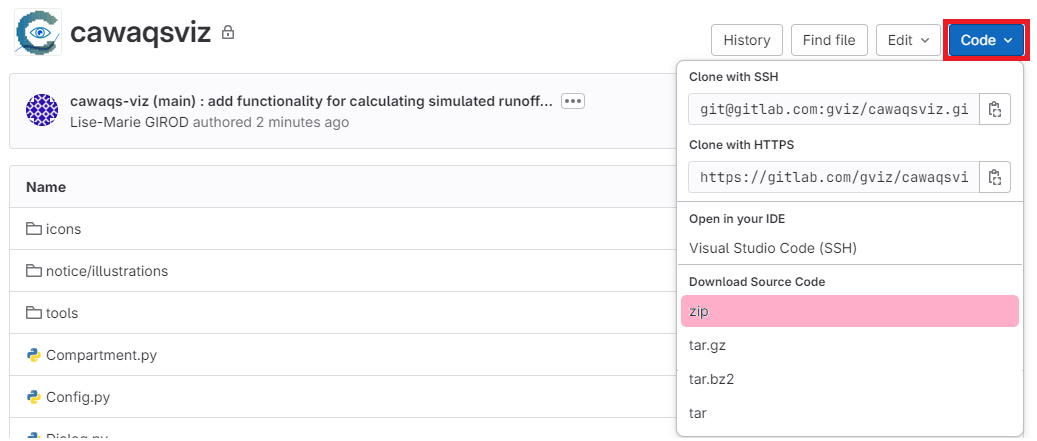
\includegraphics[width=0.8\linewidth]{1_installation_requirements/fig/download_gitlab.png}
    \caption{Téléchargement de l'archive \cwv~depuis l'interface web de dépôt \gitlab.}
    \label{fig-download_cwv}
\end{figure}

Dans la barre supérieure de menus de QGIS, cliquez sur \gui{Extensions} puis \gui{Installer/Gérer les extensions}. La fenêtre de gestion et d'import des extensions s'ouvre. Sélectionner \gui{Installer depuis un ZIP} (\cref{fig-QGIS_install_from_zip}). 

\begin{figure}[H]
    \centering
    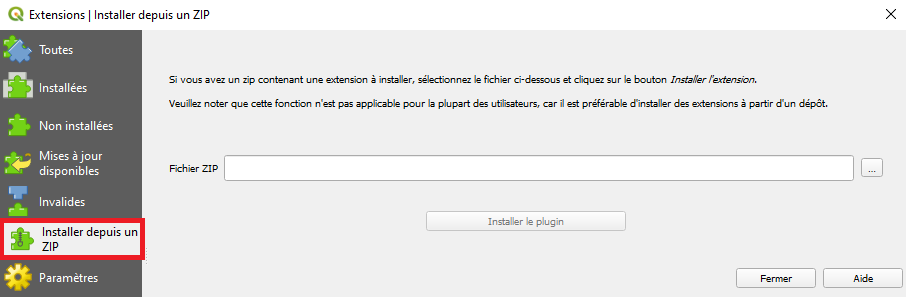
\includegraphics[width=1\linewidth]{1_installation_requirements/fig/QGIS_install_from_zip.png}
    \caption{Boîte de dialogue QGIS pour la gestion d'extensions.}
    \label{fig-QGIS_install_from_zip}
\end{figure}

Une fois le fichier \script{.zip} décompressé sous QGIS, il peut être nécessaire d'activer ce dernier dans la même fenêtre de gestion des extensions en naviguant dans le volet \gui{Installées}. L'extension \cwv~doit être cochée pour figurer dans la barre d'outils QGIS (\cref{fig-CWV-activation}).

\begin{figure}[H]
    \centering
    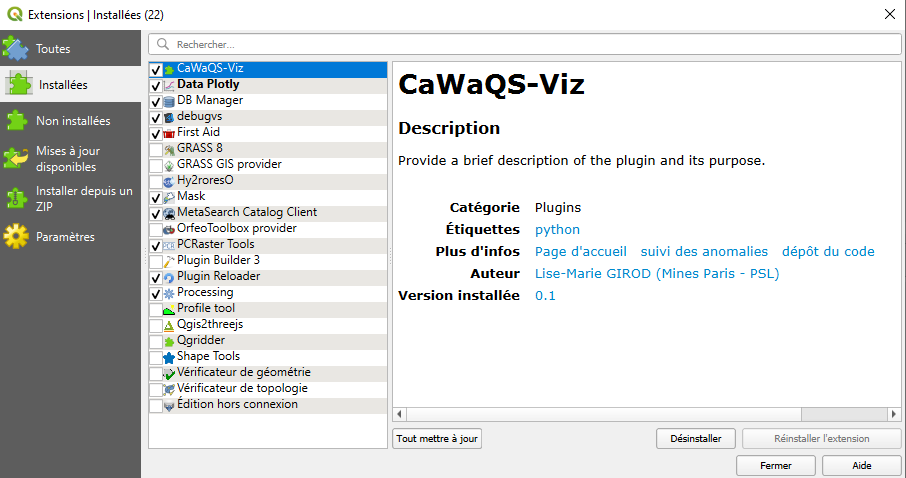
\includegraphics[width=1\linewidth]{couverture/fig/QGIS_get_plugin_in_toolbar.png}
    \caption{Activation de l'extension \cwv~dans l'application QGIS.}
    \label{fig-CWV-activation}
\end{figure}

Une fois l'application présente dans la barre d'outils de QGIS, celle-ci est prête à être lancée d'un simple clic sur l'icône 
\includegraphics[height=0.45cm]{couverture/fig/Icon_CaWaQSVIZ.png}.

\alertinfo{Pour utiliser toute nouvelle mise à jour du plug-in dans QGIS, il sera nécessaire de réitérer l'intégralité de cette procédure (\cref{sec-install-user}).}

\section{Installation pour les développeurs} \label{sec-install-expert}

Le répertoire de dépôt \gitlab~de \cwv~peut être cloné depuis un terminal de commande : 

\begin{lstlisting}[language=bash]
$ git clone https://gitlab.com/gviz/cawaqsviz
\end{lstlisting}

Le répertoire de l'application doit être placer à l'emplacement (dossier) des applications natives de QGIS afin que toute modification du code source du plug-in puisse être prise en compte par QGIS lors de son démarrage. Le répertoire QGIS est accessible \textit{via} le chemin suivant :

\begin{lstlisting}[language=bash]
#windows
C:/Programmes/QGIS3.X.X.X/apps/qgis-ltr/python/plugin/
#linux 
/home/bin/QGIS3.X.X.X/apps/qgis-ltr/python/plugin/
\end{lstlisting}


La structure du code du plug-in est décrite en chapitre \ref{chap-description-src}.\\

\alertinfo{L'autocomplétion des fonctionnalités liées à la libraire qgis est diponible à condition d'utiliser l'interpréteur python utilisé par QGIS. Un environnement virutel peut-être initalisé à cet effet.}

\textbf{N.B.} : Pour faciliter le développement du plug-in, les utilitaires suivants peuvent être installés depuis le gestionnaire des applications QGIS :
\begin{enumerate}
    \item \textbf{Reloader} permet de recharger le plug-in sans relancer QGIS à chaque modification de code, 
    \item \textbf{FirstAid} permet une visualisation détaillée des erreurs retournées par l'interpréteur Python de QGIS ainsi que les différents objets et variables liées à l'extension. 
\end{enumerate}


    \chapter{Fonctionnalités et configuration de l'extension CaWaQS-Viz}
\label{chap-user}

\renewcommand{\headrulewidth}{0.3pt}
\fancyhead[LE]{\thepage} \fancyhead[RE]{\nouppercase{\textbf{\leftmark}}}
\fancyhead[RO]{\thepage} \fancyhead[LO]{\nouppercase{\textbf{\rightmark}}}
\fancyfoot[L,C,R]{}

\setlength{\parindent}{0.35cm}

\minitoc
\newpage
\

\newpage

% ================================================================

\section{Généralités}
\label{sec-generalites}

L'extension \cwv~intègre plusieurs fonctionnalités accessibles depuis sa boîte de
dialogue d'accueil (\cref{fig-cwv_home_page}) :
\begin{itemize}
    \item une entrée dédiée à la configuration de l'application \cawaqs~(\gui{Settings}
        - \cref{sec-config} à \ref{sec-json_config_project}) ;

    \item des outils d'aide à la calibration (\gui{Calibration tools} - \cref{sec-calib-tools})
        ;

    \item des fonctionnalités de visualisation des chroniques temporelles de débits
        et de piézométrie simulées et observées (\gui{Compare Sim/Obs} - \cref{sec-com-simobs})
        ;

    \item des outils de visualisation de la distribution spatiale des composantes
        hydrologiques (\gui{Spatial Maps} - \cref{sec-spatial-map}) ;

    \item une fonction de visualisation du bilan hydrologique (\gui{Budget Bar Plot}
        - \cref{sec-bufget-barplot}) ;

    \item un visualiseur des régimes hydrologiques (\gui{Hydrological regime} - \cref{sec-regime-hydro}).
\end{itemize}

\begin{figure}[H]
    \centering
    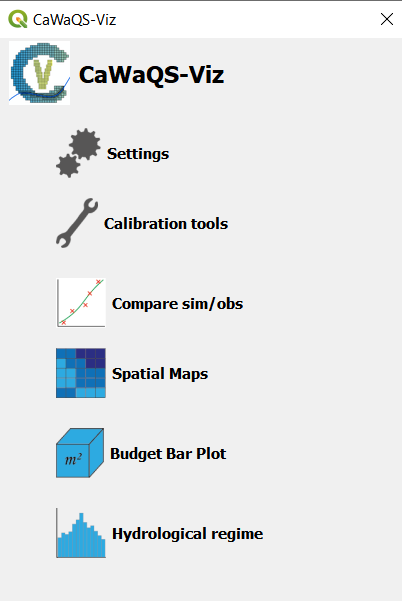
\includegraphics[width=0.4\linewidth]{
        2_application_user_guide/fig/CAWAQS_VIZ_home_page.png
    }
    \caption{Boîte de dialogue d'accueil de l'application \cwv.}
    \label{fig-cwv_home_page}
\end{figure}

\section{Configuration du plug-in \cwv}
\label{sec_config}

L'utilisation de l'extension \cwv~se fonde sur un projet \script{SIG} préexistant
contenant :
\begin{itemize}
    \item les maillages des différents modules de l'application \cawaqs, aux
        résolutions des sorties de modélisation ;

    \item les points d'observation et/ou les points d'extractions, situés dans les limites de l'emprise du modèle.
\end{itemize}

Le plug-in doit être configuré pour lire les différents fichiers de sortie de modélisation
et/ou d'entrée \cawaqs~ainsi que les différents maillages. Cette paramétrisation
du plug-in peut être effectuée dans la fenêtre \gui{Settings}. Pour ce faire, deux
procédures sont possibles :
\begin{itemize}
    \item importer un fichier de configuration \script{.json} préalablement
        établi ;

    \item configurer manuellement le projet dans la deuxième partie de la boîte de
        dialogue de la figure \ref{fig-DialogSettings}.
\end{itemize}

\begin{figure}[H]
    \centering
    % Première figure
    \begin{subfigure}
        [b]{0.45\linewidth}
        \centering
        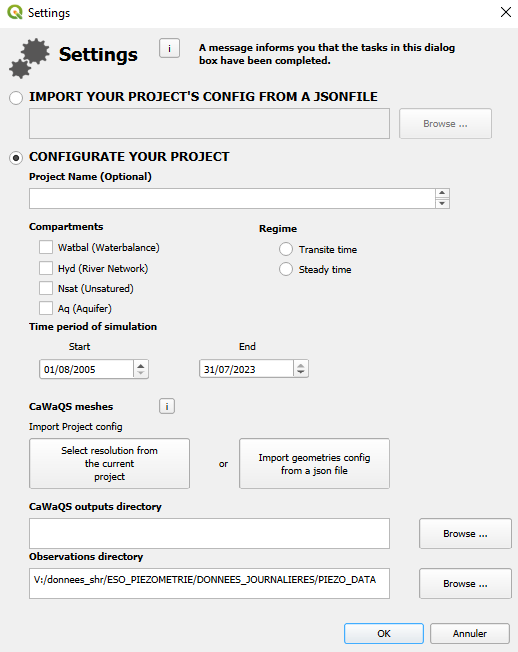
\includegraphics[width=\linewidth]{
            2_application_user_guide/fig/DialogSettings_creat_project.png
        }
        \caption{}
        \label{fig_DialogSettings_creat_projet}
    \end{subfigure}
    \hfill
    % Deuxième figure
    \begin{subfigure}
        [b]{0.45\linewidth}
        \centering
        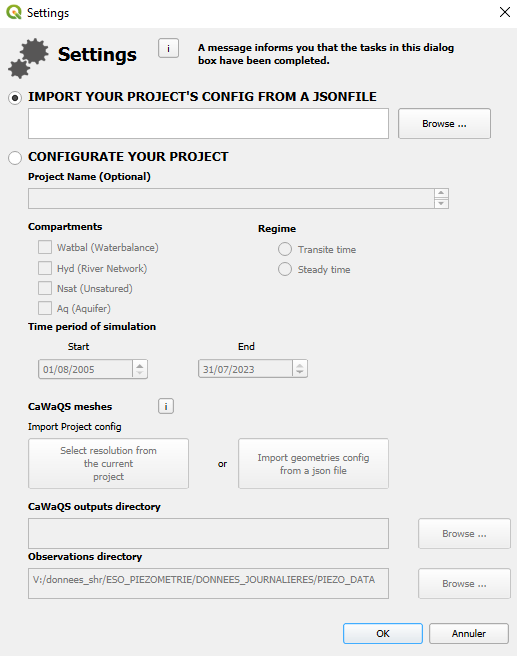
\includegraphics[width=\linewidth]{
            2_application_user_guide/fig/DialogSettings_import_project.png
        }
        \caption{}
        \label{fig_DialogSettings_inport_projet}
    \end{subfigure}
    \caption{Boîte de dialogue \gui{Settings} du plug-in. La méthode de
    configuration de l'application \cwv doit être sélectionnée : \textbf{(a)} création
    d'un nouveau projet \textbf{(b)} importation d'une configuration de projet. }
    \label{fig-DialogSettings}
\end{figure}

Les détails de ces deux procédures de configuration de l'application sont décrits
respectivement en paragraphes \ref{sec-config-manual} et \ref{sec-json_config_project}.

\section{Configuration manuelle du plug-in : première utilisation}
\label{sec-config-manual}

La partie inférieure de la boîte de dialogue \gui{Settings} permet de configurer
manuellement le plug-in. Les éléments suivants doivent y être définis :
\begin{enumerate}
    \item un nom de projet ;

    \item les compartiments modélisés ;

    \item une configuration des couches SIG des maillages ;

    \item les répertoires de sortie de modélisation et d'observation\footnote{les répertoires d'observation des débits et de piézométrie sont supposés être dans le même répertoire parent.} si des points d'observation sont définis dans le projet.
\end{enumerate}

Le nom du projet sera utilisé pour nommer un sous-dossier créé dans le répertoire
de post-traitement. Les sorties graphiques de l'application \cwv\ seront placées
dans ce dossier de post-traitement.\\

La configuration des géométries peut également être importée depuis un fichier de
configuration \json~(en cliquant sur \gui{Importer une configuration des géométries depuis un \json})
ou définie manuellement \textit{via} l'option \gui{Sélectionner les résolutions depuis le projet courant}.

\alertinfo{À noter que toute configuration manuelle de projet et de géométrie sera exportée au format \json~dans le répertoire de post-traitement à l'exécution de la boite de dialogue \gui{Settings}.}

\subsection{Contenu du projet QGIS utilisé pour l'exploitation des résultats de
simulations \cawaqs}
\label{sec-res-cawaqs}

\textbf{{Les \script{shapefiles} des maillages du modèle \cawaqs}}\\
Le projet QGIS utilisé pour le traitement des simulations avec l'utilitaire \cwv
nécessite de contenir :
\begin{itemize}
    \item les maillages (résolutions) des compartiments au format \gui{shapefile}
        du modèle (se référer à la notice \cawaqs~\footnote{Terminologie de
        géométrie \cawaqs. Pour plus d'informations sur les différents types de maillages,
        se référer aux notices du modèle (\ie~notice utilisateur et guide technique),
        disponibles sur le dépôt GitLab \href{https://gitlab.com/cawaqs/cawaqs}{https://gitlab.com/cawaqs/cawaqs}.}
        pour identifier les résolutions de sorties du compartiment \gui{WATBAL}).
        Les types de résolution \cawaqs~à importer dans le projet SIG en vue d'un
        traitement des sorties de modélisation sont fonction des compartiments
        effectivement modélisés ;

    \item les points d'observation des compartiments à définir dans l'extension \cwv.
\end{itemize}

\begin{table}[H]
    \centering
    \begin{tabular}{>{\raggedleft\arraybackslash}m{3cm}|>{\centering\arraybackslash}m{3.2cm}>{\centering\arraybackslash}m{3.2cm}>{\centering\arraybackslash}m{3.2cm}>{\centering\arraybackslash}m{3.2cm}}
        \hline
                                                                & \textbf{Compartiment de surface\newline(WATBAL)}                                                               & \textbf{Compartiment hydraulique \newline(HYD)} & \textbf{Compartiment non saturé \newline(NSAT)} & \textbf{Compartiment aquifère \newline(AQ)} \\
        \hline
        \textbf{Résolution \cawaqs}                             & Maille unitaire de surface (\texttt{ele\_bu})\footnotemark~ \newline ou Cellule de production (\texttt{Cprod}) & Élément rivière (\texttt{ele\_musk})            & Grille du milieu non saturé                     & Maillages de toutes les couches aquifères   \\
        \hline
        \textbf{Champs obligatoires dans la table attributaire} & Identifiants des cellules                                                                                      & Identifiants GIS des éléments rivières          & Identifiants des mailles                        & Identifiants absolus des mailles            \\
        \hline
    \end{tabular}
    \caption{Résolutions \cawaqs~pouvant être importées comme résolution de
    compartiment.}
    \label{tab-resolution_per_compartment}
\end{table}

\alertwarning{Les noms des couches SIG du projet correspondant aux aquifères doivent être identiques à ceux définis dans la configuration CaWaQS afin d'assurer le bon fonctionnement de l'application.}

\textbf{{Les \script{shapefiles} des points d'extractions}}\\

L'extraction des simulations de débit et de charge hydraulique peut être réalisée
aux droits de point d'extraction. Deux types types de points d'extraction peuvent être
renseignés :
\begin{itemize}
    \item des points d'extraction simple, qui n'intègrent pas de chronique de
        mesure ;

    \item des points d'observation, qui sont des points d'extraction avec des
        données de mesure.
\end{itemize}

Les points d'extraction et d'observation sont contenus dans deux fichiers
\script{shapefile} distinct dont les tables attributaires contiennent les champs
recensé dans la table \ref{tab_obs_extract}.

\vspace{8pt}

\renewcommand{\arraystretch}{1.5} % pour aérer les lignes
\newcolumntype{C}[1]{>{\centering\arraybackslash}p{#1}} \newcolumntype{C}[1]{>{\centering\arraybackslash}p{#1}}

\begin{table}[H]
    \begin{tabular}{|C{0.2\textwidth}|C{0.35\textwidth}|C{0.35\textwidth}|}
        \hline
        \textbf{TYPE DE POINT}& \textbf{CONTENUS DE LA TABLE ATTRIBUTAIRE} & \textbf{RENDUS} \tabularnewline                    \hline
        \textbf{Point d’extraction}  & 
        \begin{itemize}[leftmargin=*, itemsep=0.5ex]
            \item Nom du point
            \item Identifiant de la maille de rattachement\footnote{\gui{ID GIS} si extraction dans le compartiment HYD, \gui{ID ABS} si extraction en aquifère, champ optionnel}, identifiant de la couche aquifère (si extraction en aquifère)\end{itemize} & \begin{itemize}[leftmargin=*, itemsep=0.5ex]\item Hydrogrammes et courbes piézométriques simulés au droit du point d’extraction\end{itemize} \tabularnewline                     \hline
        \textbf{Point d’observation} & 
        \begin{itemize}[leftmargin=*, itemsep=0.5ex]
            \item Nom du point
            \item Identifiant de la maille de rattachement \footnotemark[\value{footnote}]
        \end{itemize} & 
        \begin{itemize}[leftmargin=*, itemsep=0.5ex]
            \item Hydrogrammes et courbes piézométriques simulés et observés
            \item Critères objectifs de comparaison entre les observations et les simulations
        \end{itemize} \tabularnewline \hline
    \end{tabular}
    \label{tab_obs_extract}
    \caption{Structure des couches SIG relatives aux points d’extraction et rendus graphiques associés}
\end{table}

\vspace{8pt}

\alertwarning{Les \script{shapefile} d'observation doivent être importée dans le projet et renseignée dans la configuration de \cwv~si les compartiements HYD et/ou AQ sont traités. Sans observations l'extention ne sera pas fonctionnelle}

\subsection{Configuration de la géométrie du projet depuis un projet QGIS
existant}
\label{sec_config_manuelle}

La configuration géométrique de l'application \cwv peut être définie depuis un projet
QGIS existant via la boite de dialogue \gui{Application configuration from an existing projet}
de la boite de dialogue de paramétrage de l'application.

La fenêtre est organisée selon deux sections :
\begin{itemize}
    \item sur la gauche, sont listés les compartiments \cawaqs (WATBAL, HYD, AQ,
        NSAT),

    \item sur la droit, sont listé les paramètres à définir pour produire les
        rendus graphique (débit et piézométrie) aux droits de points d'observation
        (point d'extraction avec observation) ou de points d'exctration (sans observation).
\end{itemize}

Si les champs de paramétrage de l'application sont laissé vide, le compartiment
concerné n'est pas intégrer dans la configuration géométrique. \\

Les champs des compartiments sont configurés suivant :\\

\noindent
\textbf{Le compartiment de surface (\gui{"WATBAL COMPARTMENT"}) :}

\vspace{0.5em}

\begin{minipage}[t]{0.45\textwidth}
    \begin{itemize}
        \item \gui{Surface resolution} : résolution de sortie du bilan hydrique de surface (CPROD ou elebu) ;
        \item \gui{cell id} : le numéro de la colonne dans la table attributaire qui correspond à l'identifiant des mailles ;
        \item \gui{cell area} : le numéro de la colonne dans la table attributaire qui correspond à la surface des mailles (paramètre optionnel).
    \end{itemize}
\end{minipage}%
\hfill
\begin{minipage}[t]{0.45\textwidth}
    \centering
    \raisebox{\dimexpr-\height+\ht\strutbox}{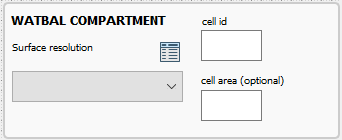
\includegraphics[
        width=0.8\linewidth
    ]{
        2_application_user_guide/fig/DialogSelectLayer_watbal.png
    }} \captionof{figure}{Champ de paramétrage du compartiment WATBAL}
\end{minipage}

\vspace{1em}
\textbf{Le compartiment hydrologique (\gui{HYD COMPARTMENT})}

\begin{minipage}[t]{0.45\textwidth}
    \begin{itemize}
        \item \gui{Hyd resolution} : nom de la résolution de sortie du compartiment \gui{HYD} (éléments rivières) ;
        \item \gui{GIS Id} : le numéro de la colonne dans la table attributaire qui correspond à l'identifiant GIS des mailles 
    \end{itemize}
\end{minipage}%
\hfill
\begin{minipage}[t]{0.45\textwidth}
    \centering
    \raisebox{\dimexpr-\height+\ht\strutbox}{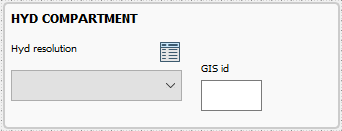
\includegraphics[
        width=0.8\linewidth
    ]{
    2_application_user_guide/fig/DialogSelectLayer_hyd.png
    }} 
    \captionof{figure}{Champ de paramétrage du compartiment HYD}
\end{minipage}

\vspace{1em}
\textbf{Le compartiment non saturé (\gui{NSAT COMPARTMENT}):}

\begin{minipage}[t]{0.45\textwidth}
    \begin{itemize}
        \item \gui{Unsatured zone resolution} : nom de la résolution de sortie du compartiment \gui{NSAT} ;
        \item \gui{cell id} : le numéro de la colonne dans la table attributaire qui correspond à l'identifiant des mailles. 
    \end{itemize}
\end{minipage}%
\hfill
\begin{minipage}[t]{0.45\textwidth}
    \centering
    \raisebox{\dimexpr-\height+\ht\strutbox}{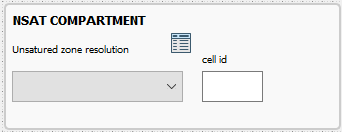
\includegraphics[
        width=0.8\linewidth
    ]{
    2_application_user_guide/fig/DialogSelectLayer_nsat.png
    }} 
    \captionof{figure}{Champ de paramétrage du compartiment HYD}
\end{minipage}

\vspace{1em}
\textbf{Le compartiment saturé (\gui{AQ COMPARTMENT})}

\begin{minipage}[t]{0.45\textwidth}
     \begin{itemize}
            \item \gui{Aquiferes resolutions} : les couches SIG constituant le
                maillage souterrain. La couche sélectionnée est ajoutée en cliquant
                sur \gui{Add}. Les couches doivent être ordonnées de la couche supérieure
                à la couche inférieure à l'aide des boutons \gui{up} et \gui{down}.
                Enfin, une couche peut être supprimée de la liste en cliquant sur
                \gui{remove} ;
            \item \gui{cell id abs} : identifiant de la colonne de la table
                attributaire contenant l'identifiant absolu des mailles. Cet identifiant
                peut être homogène entre les couches SIG : dans ce cas, \gui{homogeneous ID ABS}
                doit être sélectionné. Sinon, cliquer sur \gui{heterogeneous ID ABS}
                pour ouvrir des boîtes de dialogue permettant de renseigner, pour
                chaque couche, la colonne contenant l'ID ABS des mailles (cf. Fig \ref{fig_id_abs_hetero}).
        \end{itemize}
\end{minipage}%
\hfill
\begin{minipage}[t]{0.45\textwidth}
    \centering
    \raisebox{\dimexpr-\height+\ht\strutbox}{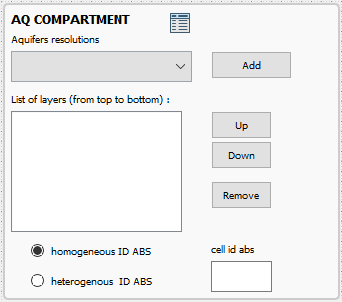
\includegraphics[
        width=0.8\linewidth
    ]{
    2_application_user_guide/fig/DialogSelectLayer_aq.png
    }} 
    \captionof{figure}{Champ de paramétrage du compartiment HYD}
    \raisebox{\dimexpr-\height+\ht\strutbox}{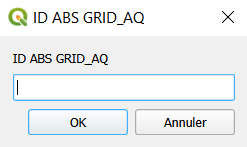
\includegraphics[
        width=0.5\linewidth
    ]{
2_application_user_guide/fig/DialogSelect_Layer_hetero_ID_ABS
    }} 
    \label{fig_id_abs_hetero}
    \captionof{figure}{Fenêtre de sélection de l'identifiant du champ contenant l'\gui{ID ABS} dans la table attributaire dans le cas d'identifiant de champ hétérogène entre les couches}
\end{minipage}



\alertwarning{Quelques point de vigilance :
\begin{itemize}
    \item \textbf{L'identifiant de la première colonne d'une table attributaire commence à 0}. L'icône 
\includegraphics[height=0.45cm]{2_application_user_guide/fig/table.png} permet de visualiser les identifiants des champs renseignés dans la table attributaire de la résolution sélectionnée dans la liste déroulante ;
    \item le code (ex : code BSS) d'un point d'observation doit être \textbf{unique} entre tous les points d'observation ;
    \item La configuration géométrique des compartiments cochés dans la boite de dialogue de paramétrisation du projet, doit être définie dans la boite de dialogue de configuration des géométries.
\end{itemize}}

\vspace{8pt}

\textbf{Les points d'extraction - \gui{Hydrological and Hydrological plots}} \\
Les points d'extraction peuvent être de deux types :
\begin{itemize}
    \item[$\bullet$] des points d'extractions simples, qui permettent de
    visualiser des variables simulées au droit d'un point de ces derniers ;
    \item[$\bullet$] des points d'observation, qui permettent de comparer les variables simulées à des données d'observation aux droits de ces derniers.
\end{itemize}



La configuration des points d'extraction nécessite de renseigner dans les champs \gui{GIS Layer}, la nom de la couche dans le projet QGIS contenant les points d'observations et les points d'extraction selon le compartiment \cws~ concerné. Les identifiants des champs à renseigner sont les suivants : 
\vspace{8pt}

\begin{minipage}[t]{0.45\textwidth}
    \textbf{Les points d'extraction du compartiment \gui{HYD}} 
    \vspace{4pt}

     \underline{Les points d'extraction}

    \begin{itemize}
        \item \gui{name} : nom du point d'observation ;
        \item \gui{ID GIS} : identifiant GIS du point d'observation auquel le point d'observation doit être attaché (champ optionnel)
    \end{itemize}

    \vspace{2pt}
    \underline{Les points d'observation} 
    \begin{itemize}
        \item \gui{code} : code d’identification du points d'observation, doit être un code unique pour chaque point. Le fichier d'observation du point doit porte le même nom sous l’extension \script{.dat} ;
        \item les champ \gui{name} et \gui{ID GIS} sont également préciser pour la configuration des points d'observation 
    \end{itemize}
    \vspace{8pt}
    \textbf{Les points d'extraction du compartiment \gui{AQ}} 
    \vspace{4pt}

     \underline{Les points d'extraction}

    \begin{itemize}
        \item \gui{name} : nom du point d'observation ;
        \item \gui{ID LAYER} : identifiant de la couche aquifère
        \item \gui{ID GIS} : identifiant GIS du point d'observation auquel le point d'observation doit être attaché (champ optionnel)
    \end{itemize}

    \vspace{2pt}
    \underline{Les points d'observation} 
    \begin{itemize}
        \item \gui{code} : code d’identification du points d'observation, doit être un code unique pour chaque point. Le fichier d'observation du point doit porté le même nom sous l’extension \script{.dat} ;
        \item les champ \gui{name} et \gui{ID GIS} sont également préciser pour la configuration des points d'observation 
    \end{itemize}

    
\end{minipage}%
\hfill
\begin{minipage}[t]{0.45\textwidth}
    \centering
    \raisebox{\dimexpr-\height+\ht\strutbox}{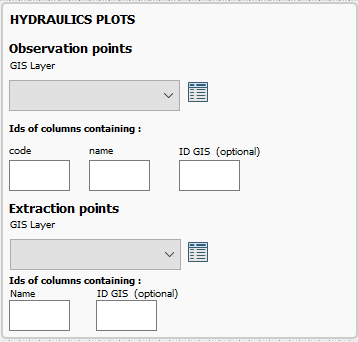
\includegraphics[
        width=0.9\linewidth
    ]{
    2_application_user_guide/fig/DialogSelectLayer_hyd_extraction.png
    }} 
    \captionof{figure}{Champs de configuration des points d'extraction du compartiment \gui{HYD}}
    \vspace{4pt}
    \raisebox{\dimexpr-\height+\ht\strutbox}{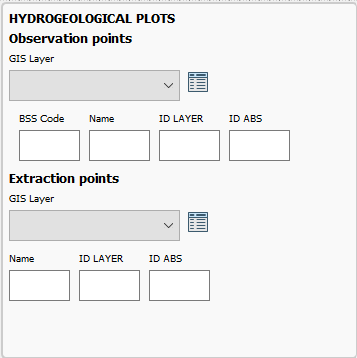
\includegraphics[
        width=0.9\linewidth
    ]{
    2_application_user_guide/fig/DialogSelectLayer_aq_extraction
    }} 
    \label{fig_id_abs_hetero}
    \captionof{figure}{Champs de configuration des points d'extraction du compartiment \gui{AQ}}
\end{minipage}

\alertwarning{
Le points d'extraction doivent être contenus dans un fichier \script{.shp} différent des points d'observtion. Les points ne peuvent pas être contenu dans le même fichier s'il s'agit d'extraction dans deux compartiment différent.
}


\alertinfo{
Une sauvegarde préliminaire du fichier de configuration géométrique peut être sauvegardé en renseignant un chemin de fichier dans le champ situé en bas à gauche de la boite de dialogue. Ce fichier (\cfcod \ref{code_config_geom})  sera enregistré à l'exucution de la boite de dialogue \gui{Settings} si le  si le projet configuré n'existe pas encore dans le répertoire
de post-traitement renseigné. 
Plusieurs configurations de projet peuvent être sauvegardées dans un même répertoire de post-Processing, sous réserve qu'elles n'aient
pas le même nom de projet. }



\subsection{Configuration des résolutions depuis un fichier de configuration
\json}

La configuration géométrique des résolutions peut être renseignée par un fichier
\json\ selon la structure suivante :

\begin{lstlisting}[language=json, caption={Contenu d'un fichier de configuration géométrique}, label={code_config_geom}]
{   // liste des compartiments CaWaQS a analyser (1 = AQ, 2 = HYD, 3 = WATBAL) 
    "ids_compartment": [], 
                           
    "resolutionNames": 
    {
        "1": 
            [[""]], // liste des noms des maillages aquiferes dans le projet QGIS 
        "2" : 
            [[""]], // liste du nom du maillages riviere dans le projet QGIS 
        "3" : 
            [[""]] // liste du nom du maillage de surface dans le projet QGIS 
        "4" : 
            [[""]] // liste du nom du maillage du non-sature dans le projet QGIS 
        }, 
    "ids_col_cell": { // "id compartiment" : "no de la colonne de l'id des mailles"
        "1" : "",  // "id AQ" : "no de la colonne de l'id absolue"
        "2" : "",  //"id HYD" : "no de la colonne de l'id GIS"
        "3" : ""   // "id WATBAL" : "no de la colonne de l'id de la maille"
        }, 
    "obsNames": { 
    // "id compartiment" : "nom du shp des obs associes dans le projet QGIS"
        "1": "", 
        "2" : ""
        }, 
    "obsIdsColCells": {
    // "id compartiment" : "no du champ du code du point de mesure"
        "1": "", 
        "2": ""
        }, 
    "obsIdsColNames": { 
    // "id compartiment" : "no du champ du nom du point de mesure"
        "1": "", 
        "2" : ""
        }, 
    "obsIdsColLayers": { 
    // "id compartiment" : "no du champ de l'identifiant de la couche aquifere"
        "1": "", 
        "2" : null
        }, 
    "obsIdsCell": { 
    // "id comp." : "no du champ de l'id absolu ou gis de maille ratachee a l'obs
        "1" : "", 
        "2" : null
    }, 
     "extNames": {
    // "id compartiment" : " nom du shp d'extraction associes dans le projet QGIS "
        "2": "",
        "1": ""
    },
    "extIdsColNames": {
    // "id compartiment" : "no du champ contenant le nom du point d'extraction"
        "2": "",
        "1": ""
    },
    "extIdsColLayers": {
    // "id compartiment" : "no du champ contenant l'identifiant de la couche aquifere"
        "2": null,
        "1": ""
    },
    "extIdsColCells": {
    // "id compartiment" : "no du champ contenant l'identifiant de la maille"
        "1": "",
        "2": "",
    }
}
}
\end{lstlisting}

\subsection{Contenu du répertoire de post-traitement}

À l'exécution de la boîte de dialogue de paramétrage de l'application \cwv, le
sous-répertoire du projet est créé dans le répertoire de post-traitement indiqué.
Si le projet n'existe pas encore dans ce répertoire, un sous-répertoire au nom
du projet sera créé, contenant les fichiers de configuration du projet et des résolutions,
écrits au format \gui{json}.

\section{Configuration du projet depuis un fichier de configuration projet \json}
\label{sec-json_config_project}

L'import d'un fichier externe \json~peut également être utilisé pour configurer
du projet. Ce fichier est construit de la manière suivante

\begin{lstlisting}[language=json]
{
    "json_path_geometries": str,
    "projectName": str, 
    "cawOutDirectory": str,
    "startSim": int,
    "endSim": int,
    "obsDirectory": str,
    "ppDirectory": str, 
    "regime": str
}
\end{lstlisting}

\vspace{-0.6cm}
Le contenu de chaque objet de ce fichier \json~est le suivant :
\begin{itemize}
    \item \gui{json\_path\_geometries} : chemin absolu du fichier de
        configuration des résolutions ;

    \item \gui{projectName} : nom du projet ;

    \item \gui{cawOutDirectory} : chemin absolu du répertoire contenant les
        sorties de modélisation \cawaqs~;

    \item \gui{startSim} et \gui{endSim} : années de départ et de fin de la simulation
        au format \script{integer} ;

    \item \gui{obsDirectory} : chemin absolu du répertoire parent contenant les
        chroniques observées ;

    \item \gui{ppDirectory} : chemin absolu du répertoire de post-traitement. Il
        est à noter que le chemin doit être pré-existant. Le cas échéant, il ne sera
        pas créé par l'application.

    \item \gui{regime} : régime de modélisation ("Transient" ou "Steady")
\end{itemize}
    \chapter{Les fonctionnalités CaWaQS-Viz}
\label{chap-features}

\renewcommand{\headrulewidth}{0.3pt}
\fancyhead[LE]{\thepage} \fancyhead[RE]{\nouppercase{\textbf{\leftmark}}}
\fancyhead[RO]{\thepage} \fancyhead[LO]{\nouppercase{\textbf{\rightmark}}}
\fancyfoot[L,C,R]{}

\setlength{\parindent}{0.35cm}

\minitoc
\newpage
\

\newpage

% ================================================================
\alertwarning{Toutes les sorties shapefile générés par \cwv sont temporaires. Si elles ne sont pas sauvegardées, elles ne seront plus accécibles à la réouverture du projet.}

\section{\gui{Calibration Tools}: Les outils de calibration}
\label{sec-calib-tools}

La boîte de dialogue \gui{Calibration Tools} (\cref{fig_DialogCalibrationTools})
permet d'accéder aux outils de calibration du modèle \cawaqs. Ces fonctionnalités
sont les suivantes :
\begin{itemize}
    \item un outil de modification des fichiers de paramétrisation des différents
        compartiments modélisés : \gui{Modify a parametrisation file} (\cref{sec-feat-modify-param})
        ;

    \item un outil de calcul des critères de performance de calibration du modèle
        : \gui{Statistical Criteria} (\cref{sec-critstat}) ;

    \item un outil de calcul du coefficient de ruissellement simulés : \gui{Run-off coefficient calculation}
        (\cref{sec-runoff-coef}) ;

    \item un outil de visualisation des chronique simulées et observée : \gui{Compare sim/obs}
        (\cref{sec-com-simobs}).
\end{itemize}

\begin{figure}[H]
    \centering
    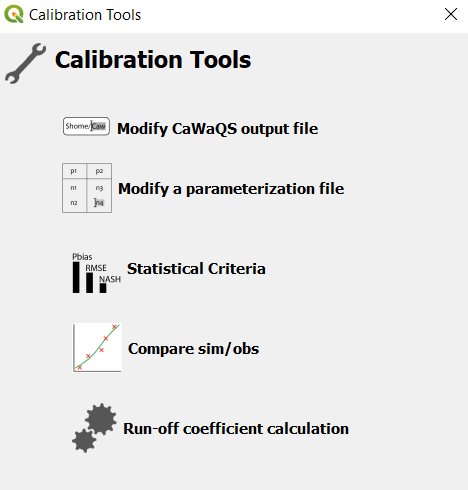
\includegraphics[width=0.65\linewidth]{
        2_application_user_guide/fig/DialogCalibrationTools.png
    }
    \caption{Boîte de dialogue des outils de calibration.}
    \label{fig_DialogCalibrationTools}
\end{figure}

\subsection{Modification des fichiers de paramétrisation}
\label{sec-feat-modify-param}

La modification des fichiers de paramétrisation peut être effectuée depuis la
boite de dialogue \gui{Modifying a parametrization file} (\cref{fig-dialog_modif_param_file}).
La résolution dépendra du fichier de calibration qui devra être sélectionné
dans le menu déroulant. L'affichage de la table se fera en cliquant sur

\includegraphics[height=0.45cm]{2_application_user_guide/fig/show.png}
. \\

Si la table attributaire affichée ne contient pas les champs du fichier de paramétrisation,
la résolution peut être liée à son fichier de paramétrisation dans la boite de
dialogue \gui{Lier la résolution à son fichier de paramétrisation} accessible en
cliquant sur
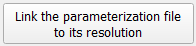
\includegraphics[height=0.55cm]{
    2_application_user_guide/fig/AccesDialogLinkParamResolution.png
}
.L'utilisation de cette boite de dialogue est décrite en \cref{sec-link_table}.

\begin{figure}[H]
    \centering
    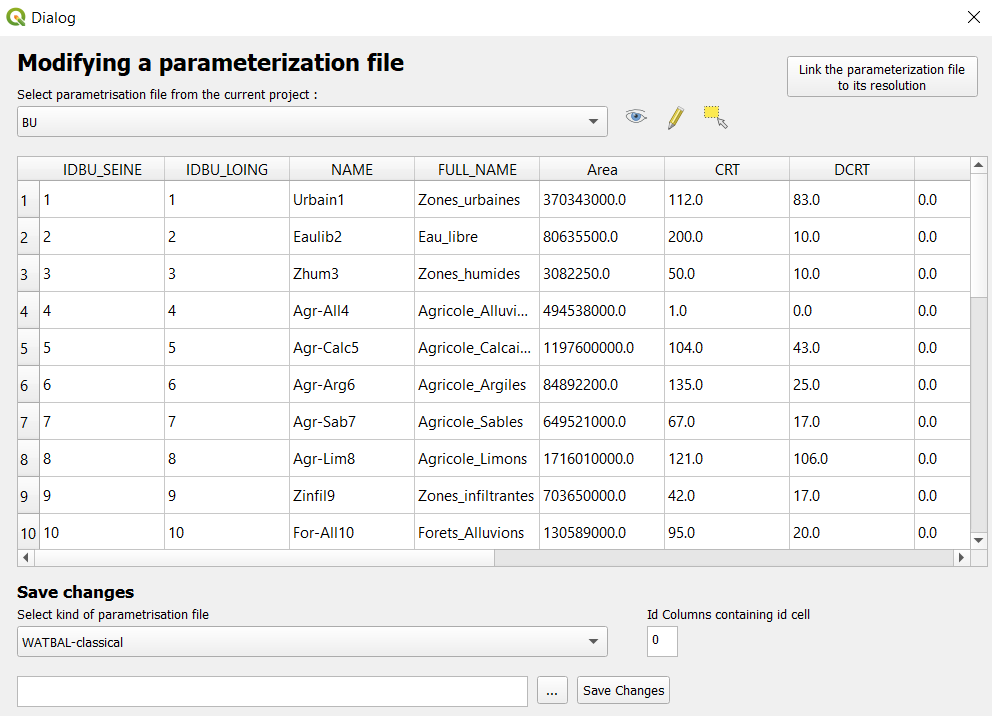
\includegraphics[width=1\linewidth]{
        2_application_user_guide/fig/DialogModifParamFile.png
    }
    \caption{Boîte de dialogue pour la modification des fichiers de
    paramétrisation.}
    \label{fig-dialog_modif_param_file}
\end{figure}

Une fois les paramètres modifiés dans la table affichée, elle peut être
enregistrée. Le nouveau chemin du fichier peut être renseigner en sélectionnant

\includegraphics[height=0.45cm]{2_application_user_guide/fig/SelectPath.png}
. Renseigner l'identifiant de la colonne contenant l'identifiant ou le nom de la
cellule \footnote{ATTENTION : Pour rappel, les identifiants des colonnes débutent
à \textbf{0}.}.

\subsection{Lier une table attributaire à sa résolution}
\label{sec-link_table}

Les paramètres du fichier de paramétrisation seront directement importés en tant
que champ de la table attributaire du fichier de la résolution concernée. Pour créer
ce lien, un type de fichier de paramétrisation doit être choisi (en fonction du compartiment
et du type de fichier de paramétrisation), la résolution \cawaqs~ainsi que le chemin
d'accès à ce fichier de paramétrisation. Différents types de fichier de
paramétrisation existent et sont répertoriés dans le tableau
\ref{tab-type_param_file}.

\begin{figure}
    \centering
    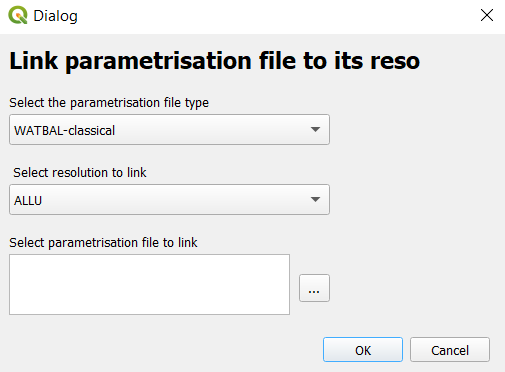
\includegraphics[width=0.7\linewidth]{
        2_application_user_guide/fig/DialogLinkTable.png
    }
    \caption{Boîte de dialogue permettant de lier une table attributaire à sa
    résolution.}
    \label{fig:enter-label}
\end{figure}

\begin{table}[H]
    \centering
    \begin{tabular}{m{4cm}|m{4cm}|m{4cm}}
        \hline
        \textbf{Compartiment} & \textbf{Type de fichier de paramétrisation} & \textbf{Paramètres renseignés dans la table}             \\
        \hline
        \script{WATBAL}       & Classical                                   & CRT, DCRT, R, FN, CQR, CQRMAX, CQI, CQIMAX et RNAP       \\
        \hline
        \script{WATBAL}       & Infiltration Excess                         & CRT, DCRT, R, FN, CQR, CQRMAX, CQI, CQIMAX, RNAP et RINF \\
        \hline
        \script{AQ}           & Transmissivity                              & T                                                        \\
        \hline
        \script{AQ}           & Storage (coefficient d'emmagasinement)      & S                                                        \\
        \hline
        \script{AQ}           & Conductance                                 & C                                                        \\
        \hline
        % Ajoutez plus de lignes de données si nécessaire
    \end{tabular}
    \caption{Les fichiers de paramétrisation pris en charge par \texttt{\cwv}.}
    \label{tab-type_param_file}
\end{table}

\subsection{\script{Statistical Criteria}: Calcul des critères statistiques de
performance au droit des points d'observation : }
\label{sec-critstat}

La boîte de dialogue \gui{Statistical Criteria} (\cref{fig-dialogstatisticalcriteria})
retourne une couche SIG suivant les géométries de la résolution d'observation
inhérente à la variable analysée. Chaque champ correspond à un critère statistique
donné. Les critères statistiques sélectionnés sont calculés sur la période
renseignée dans la partie \gui{Period for calculating statistical criteria}. \\

\subsubsection{Les critères statistiques calculé par la boite de dialogue \gui{Statistical criteria}}

\textbf{\gui{Pbias} : Bias [$\%$]}
\begin{equation*}
PBIAS = \frac{\sum(\hat{y}_i -y_i)}{\sum y_i} . 100
\quad \quad
\begin{array}{rl}
      
      y_i & : \text{variable simulée au temps $i$}\\
      O_i & : \text{variable observée au temps $i$}\\
\end{array}  
\end{equation*}

\textbf{\gui{Average SIM/OBS}}
\begin{equation*}
    A = \overline{\hat{y}} - \overline{y}
    \quad\quad
    \begin{array}{cc}
         \overline{\hat{y}} :& \text{moyenne des variables simulées} \\
         \overline{y} : & \text{moyenne des variables observées}
    \end{array}
\end{equation*}

\textbf{\gui{Nash} : Nash-Sutcliffe Model Efficiency} \citep{nash1970}
\begin{equation*}
    NSE = 1 - \frac{\sum_{i=1}^n (y_i - \hat{y}_i)^2}{\sum_{i=1}^n (y_i - \overline{y})^2}
    \quad \quad 
    \begin{array}{ll}
         y_i :& \text{variable réelle au temps } i \\
        \hat{y}_i :& \text{variable prédite au temps } i \\
    \end{array}
\end{equation*}

\textbf{\gui{RMSE} - Root Mean Squared Error} 
\begin{equation*}
RMSE = \sqrt{\frac{1}{n} \sum_{i=1}^{n} (y_i - \hat{y}_i)^2}
\quad \text{où} \quad
\begin{array}{ll}
    n :& \text{Nombre total jour de simulation} \\
    y_i :& \text{variable réelle au temps } i \\
    \hat{y}_i :& \text{variable prédite au temps } i \\
\end{array}
\end{equation*}

\textbf{\gui{KGE} - Kling-Gupta Efficiency} \citep{gupta2012}
\begin{equation}
    KGE = 1 - \sqrt{(r - 1)^2 + (\alpha - 1)^2 + (\beta - 1)^2} 
    \quad \quad
    \begin{array}{ll}
         r & : \text{coefficient de corrélation de Pearson} \\ 
         & \text{entre les série de variables simulées} \\ 
         & \text{et observées} \\
        \alpha & : \text{rapport des écarts-types simulés et observés} \\
        \beta  & : \text{biais moyen entre les séries simulées et observées}
    \end{array}
\end{equation}





Les critères suivants sont calculés automatiquement : $\overline{y}$, $\overline{\hat{y}}$, $\frac{\overline{\hat{y}}}{\overline{y}}$, $\sigma y$,  $\sigma \hat{y}$, $\frac{\sigma \hat{y}}{\sigma y}$.

\subsubsection{Sortie de la boite de dialogue \gui{Statistical Criteria}}
\label{sec_stats_crits}

La boite de dialogue génère les critères statistiques : 
\begin{itemize}
    \item aux droits des points d'observation,  
    \item à l'échelle de la couche aquifère dans le cas de simulation avec un compartiment aquifère ;
    \item à l'échelle de l'hydrosystème dans le cas de simulation avec un compartiment aquifère.
\end{itemize}
\vspace{0.3cm}

\underline{\textbf{Critères statistiques calculés aux droits des points d'observation}}\\
La boite de dialogue génère la table des critères statistiques au droit des points d'observation sous le format \script{shapefile} et \script{texte}. Le fichier Shapefile est introduit directement dans le projet \script{QGIS} courant, tandis que le fichier texte se trouvera dans le répertoire \script{../PostProcessing/STATS\_CRITS}. 
Les critères de sortie sont contenus dans les champs de chaque point de mesure sous les appels définis dans la table \ref{tab_statistical_criteria_crits_fields}.

\vspace{0.2cm}
\underline{\textbf{Critères statistiques calculés à l'échelle des unités aquifères}}\\
Dans le cas d'un calcul des critères statistiques sur le compartiment aquifère, un fichier \script{texte} enregistré dans le répertoire de \gui{Post-Processing} sous \script{../PostProcessing/STATS\_CRITS/AQ\_crits\_xxxx\_xxxx.txt}. Ce fichier recense les critères statistiques listés dans la table \ref{tab_statistical_criteria_crits_fields} défini à l'échelle de chaque unité aquifère. 

\vspace{0.2cm}
\underline{\textbf{Critère statiques calculés à l'échelle de l'hydrosystème}} \\
Les critère statistiques sont définis à l'échelle de l'hydrosystème sur la charge hydraulique en nappe. Ces critères écrits dans le fichiers \script{../PostProcessing/STATS\_CRITS/AQ\_crits\_xxxx\_xxxx.txt}. \\


\begin{table}[H]
    \centering
    \renewcommand{\arraystretch}{1.2}
    \resizebox{\textwidth}{!}{
        \begin{tabular}{rl}
        \hline
        \textbf{Nom du champ de la table de sortie} &  \textbf{Critère statistique} \\
        \hline
        \gui{NObs} & Nombre d'observations sur la période sélectionnée \\
        \gui{AObs} & Moyenne des variables observées \\
        \gui{ASIM} & Moyenne des variables simulées \\ 
        \gui{SUM\_RATIO} & Ratio de la somme des variables simulées et de la somme des variables observées \\
        \gui{StdObs} & Ecart-type des variables observées \\ 
        \gui{StdSim} & Ecart-type des variable simulées \\
        \gui{STD\_RATION} & Ratio des écart-types des variables observées et simulées \\
        \gui{PBAIS} & Biais  [\%] \\
        \gui{AVERAGE\ SIM/OBS} & Ratio moyen entre les variables simulées et observées \\
        \gui{KGE} & Kling-Gupta Efficiency \\
        \gui{NASH} & Nash-Sutcliffe Model Efficiency \\ 
        \gui{RMSE} & Root Mean Squared Error \\
        \hline
        \end{tabular}
    }
    \caption{Nom des champs des tables de sorties pour chaque critère statistique}
    \label{tab_statistical_criteria_crits_fields}
\end{table}


\begin{figure}[H]
    \centering
    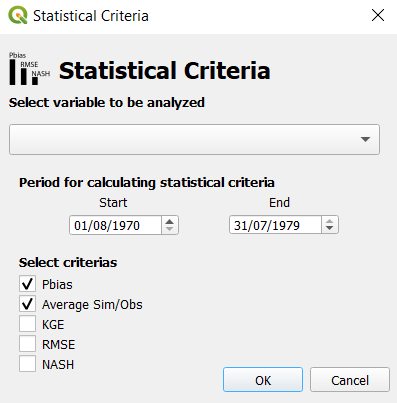
\includegraphics[width=0.5\linewidth]{
        2_application_user_guide/fig/DialogStatisticalCriteria.png
    }
    \caption{Boîte de dialogue \gui{Statistical Criteria}.}
    \label{fig-dialogstatisticalcriteria}
\end{figure}


\subsection{\script{Run-off coefficient calculation}: Calcul du coefficient de
ruissellement au droit des stations de mesure de débit}
\label{sec-runoff-coef}

Cette boîte de dialogue permet de calculer le coefficient de ruissellement simulé
et observé au droit des stations de mesures de débit. \\

\begin{figure}[H]
    \centering
    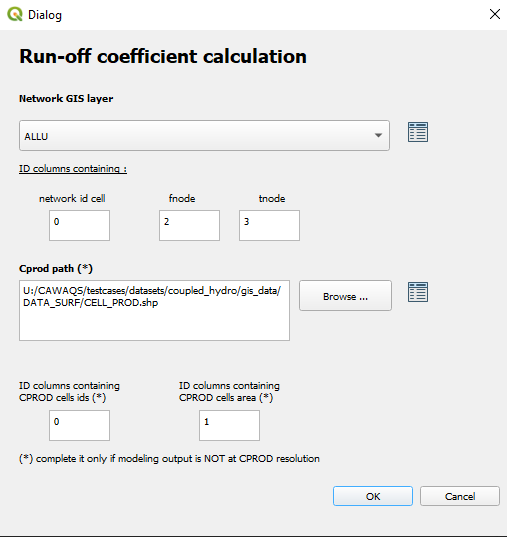
\includegraphics[width=0.5\linewidth]{
        2_application_user_guide/fig/DialogRunOffCalclulation.png
    }
    \caption{Boîte de dialogue pour le calcul du coefficient de ruissellement.}
    \label{fig-DialogRunoffCoeff}
\end{figure}

Cette boîte prend en paramètres la résolution du schéma hydrologique de surface
à l'échelle des tronçons rivières et de la résolution de surface \cawaqs~des
cellules de production (bassins versants unitaires ou \script{Cprod}). Pour la
première, le numéro de la colonne contenant les identifiants de tronçon, des
\script{Fnode} et \script{Tnode} sera à renseigner. Pour la seconde, l'identifiant
des champs contenant l'identifiant des cellules de production, d'une part, et
des surfaces de cellules. \\

Si la résolution de surface définie dans la configuration \cwv~est déjà celle
des cellules de production, dans ce cas, il ne sera pas nécessaire de renseigner
ici la partie inférieure de la boite de dialogue.

Deux nouvelles résolutions (\textit{shapefiles}) seront retournées par la boite de
dialogue et ajoutées au projet SIG courant :
\begin{itemize}
    \item \gui{CATCH} qui contient les bassin drainés par chaque station de
        mesure ;

    \item \gui{CATCH\_SURF}, produit de l'intersection entre la résolution de surface
        défini dans la configuration de \cwv~et de \gui{CATCH}. Sa table attributaire
        contient plusieurs champs :
        \begin{itemize}
            \item[$-$] \gui{CATCH\_ID} et \gui{CATCH\_SURF}: l'identifiant du
                bassin versant drainé par la station et sa surface ;

            \item[$-$] \gui{ID\_OBS} : l'identifiant la station de mesure ;

            \item[$-$] \gui{SURF\_ID} : la surface de la cellule de surface
                issue de la résolution de surface définie dans la configuration
                \cwv~;

            \item[$-$] \gui{SURF\_SURF} : sa surface ;

            \item[$-$] \gui{INTER\_ID} : l'identifiant de la cellule d'intersection
                ;

            \item[$-$] \gui{INTER\_SURF} : la surface d'intersection.
        \end{itemize}
\end{itemize}

Ces résolutions sont enregistrées au format temporaire. Il est laissé libre à l'utilisateur
de les enregistrer pour une future réutilisation. Si \cwv~reconnaît ces
résolutions dans le projet QGIS courant, elles seront réutilisées pour le calcul
des coefficients de ruissellement. \\

Ces coefficients peuvent être retrouvés dans la table attributaire de la couche d'observation
de débit renseignée à l'étape de configuration. Deux nouveaux champs sont alors
ajoutés : \gui{QruissSim} et \gui{QruissObs} désigant respectivement le
coefficient de ruissellement simulé par \cawaqs~et celui observé au droit des
stations de mesure.

\section{\script{Compare sim/obs}: Comparaison des chroniques observées et
simulées}
\label{sec-com-simobs}

Ce module de calcul permet la comparaison entre les simulations et les observations renseignées au travers de plusieurs types de rendu : 
\begin{itemize}
    \item en cliquant sur \gui{PDF printout}, un fichier \script{pdf} est généré. Les chroniques simulées et observées sont présentées avec les critères statistiques référencés dans le tableau \ref{tab_statistical_criteria_crits_fields} ;
    \item en cliquant sur \gui{Interactiv graphics}, un format \script{html} reprend le format de présentation des chroniques du format \script{pdf} de manière interactive dans le navigateur par défaut ;
    \item en cliquant sur \gui{Statistical criteria}, la boite de dialog \gui{Statistical Criteria} (\ref{sec-critstat}) s'ouvre. Les paramètres renseignés de la boite de dialogue \gui{Compare Sim-Obs} (dates, compartiement et unité de mesure des observation) sont reportés dans la boite de dialogue \gui{Statistical Criteria}. 
\end{itemize}

\begin{figure}[H]
    \centering
    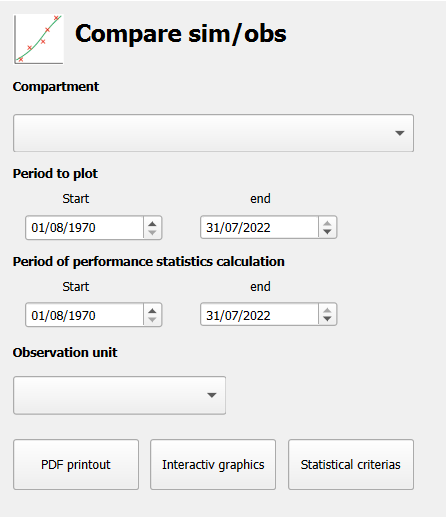
\includegraphics[width=0.45\linewidth]{
        2_application_user_guide/fig/DialogCompareSimObs.png
    }
    \caption{Fenêtre de dialogue \gui{Compare sim/obs}.}
    \label{fig-dialogCompareSimObs}
\end{figure}

Le type de compartiment (\script{AQ} = aquifère et \script{HYD} = réseau
hydrographique) est à sélectionner dans la liste déroulante située dans la partie
supérieure de la boite de dialogue (\cref{fig-dialogCompareSimObs}). Les
périodes d'impression des séries temporelles ainsi que celles du calcul des
critères statistiques sont également à renseigner. L'unité des observations de débit, utilisée pour l'exploitation des simulations du compartiment \gui{HYD} est à préciser dans le menu déroulant \gui{Observation unit}. Elle est optionnelle pour l'exploitation du compartiment \gui{AQ}. \\

Un message d'information sera affiché dans l'interface QGIS à la fin de l'exécution
de cette tâche et pointera le répertoire de post-traitement. Les fichiers
\script{.pdf} issus de l'analyse du compartiment \script{HYD} seront nommés par
défaut \gui{SIM\_OBS\_HYD.pdf}. Ceux issus de l'analyse du compartiment aquifère
seront nommés \gui{SIM\_OBS\_AQ.pdf}. Chaque page de ce document correspond à
une station de mesure.

\section{\script{Spatial Map}: Cartographie spatiale des variables hydrologiques}
\label{sec-spatial-map}

Cet outil spatialise le bilan hydrique de surface sous format \script{.shp}. Le bilan peut être produit à une fréquence annuelle, mensuelle ou journalière (à renseigner dans le champ \script{frequence}). L'agrégation temporelle peut être réalisée par une moyenne, une somme, un maximum ou un minimum (à renseigner dans le champ \script{agregator}).


\begin{figure}[H]
    \centering
    \begin{subfigure}
        [b]{0.48\linewidth}
        \centering
        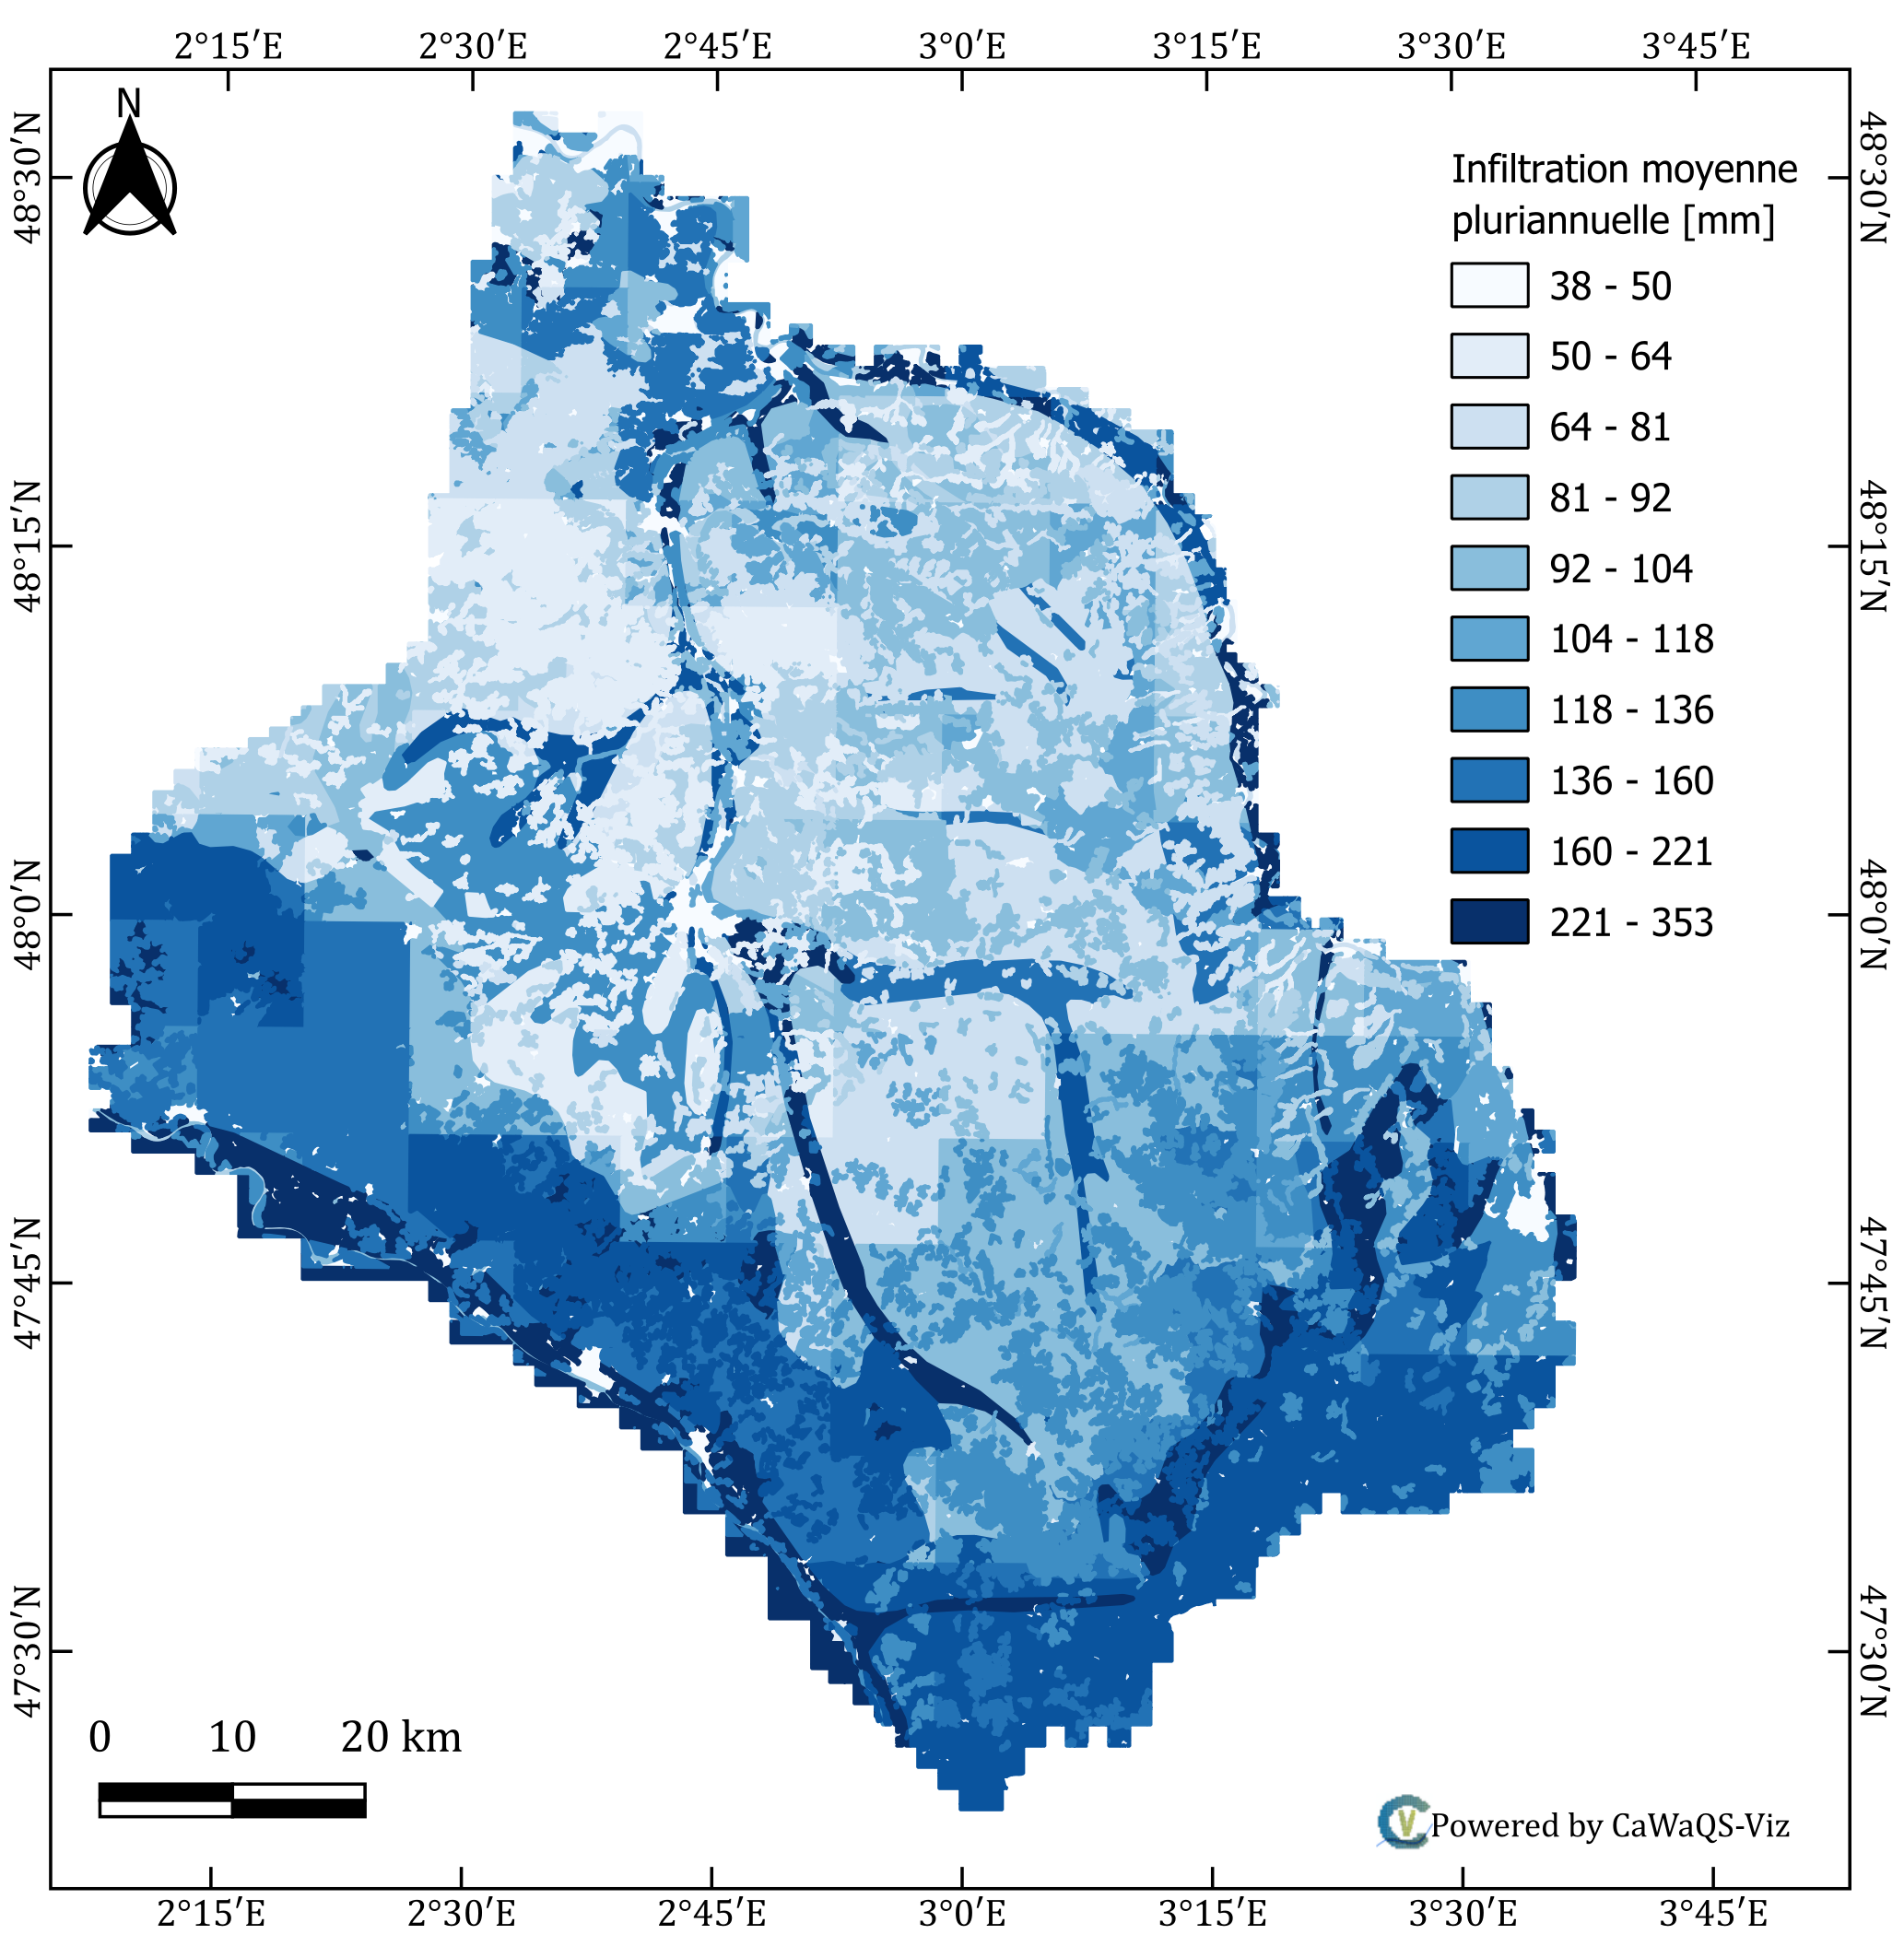
\includegraphics[width=\linewidth]{3_features/fig/OutputSpatialMap.png}
        \caption{}
        \label{fig-outSpatialMap-surf}
    \end{subfigure}
    \begin{subfigure}
        [b]{0.45\linewidth}
        \centering
        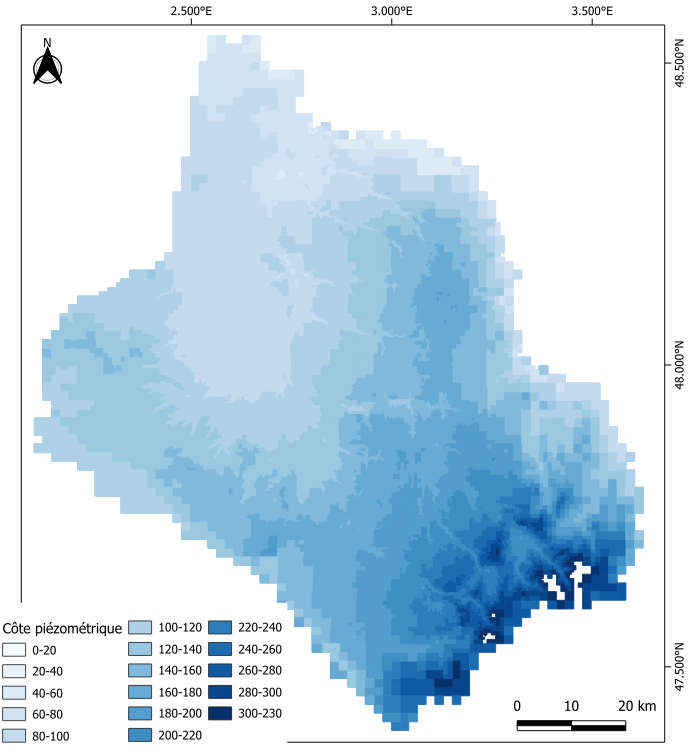
\includegraphics[width=\linewidth]{3_features/fig/Cote_piezo.png}
        \caption{}
        \label{fig-outSpatialMap-sout}
    \end{subfigure}
    \caption{Spatialisation du flux d'infiltration moyen interannuel [$mm$] (a)
    et de la piézométrie [$mNGF$] (b) simulé à l'échelle de l'hydrosystème du
    Loing }
    \label{fig:two_figures}
\end{figure}

Les valeurs prises par la variable hydrologique à spatialiser sont contenues dans
la table attributaire de la résolution \script{.shp} de sortie. La table a pour
colonnes les identifiants des années pour une agrégation annuelle, les identifiants des
mois pour une agrégation mensuelle et enfin la date pour une sortie des variables
à pas de temps journalier. Une agrégation pluriannuelle moyenne est également
possible en cochant la case \script{Pluriannual}, établissant ainsi un bilan
pluriannuel ou mensuel pluriannuel.

\begin{itemize}
    \item \script{WATBAL} : les variables de précipitations, ETR, ruissellement
        et infiltration (\ref{fig-outSpatialMap-surf}) ;

    \item \script{AQ} : les charges hydrauliques (\ref{fig-outSpatialMap-sout}), visualisables soit sur une couche
        du maillage aquifère donnée, soit sur les mailles aquifères à l'affleurement
        (maillage unique, créé par \cwv).\\
\end{itemize}

Les variables du compartiment \script{WATBAL} sont exprimées en \mmj~ou \mman~selon
le mode d'agrégation choisi. Les variables du compartiment \script{AQ} sont exprimées
en mètres.

\section{\script{Budget Bar Plot}: Visualisation du bilan hydrologique}
\label{sec-bufget-barplot}

Les bilans hydrologiques simulés peuvent être visualisés depuis cette boite de
dialogue. Ils sont construits en cohérence avec la période renseignée. Le champ
\script{Frequences} renseigne le pas de calcul du bilan hydrique (pluriannuel, annuel,
mensuel ou journalier), tandis que \script{agregator} renseigne l'agrégateur temporelle
(moyen, somme, maximum, minimum). Le bilan hydrique est aggrégé spatialement par
une moyenne des variables hydrologiques sur l'ensemble des mailles de surface.

À l'exécution de cette boîte de dialogue, une page \script{HTML} s'ouvre dans votre
navigateur et affiche un graphique interactif du bilan d'hydrologique. Une image
statique (cf. Fig. \ref{fig-budget-barplot}) de ce même graphique est
enregistrée dans le répertoire de post-process dans un sous-dossier \script{../BUDGET}
du répertoire de post-traitement.

\begin{figure*}[htb]
    \centering
    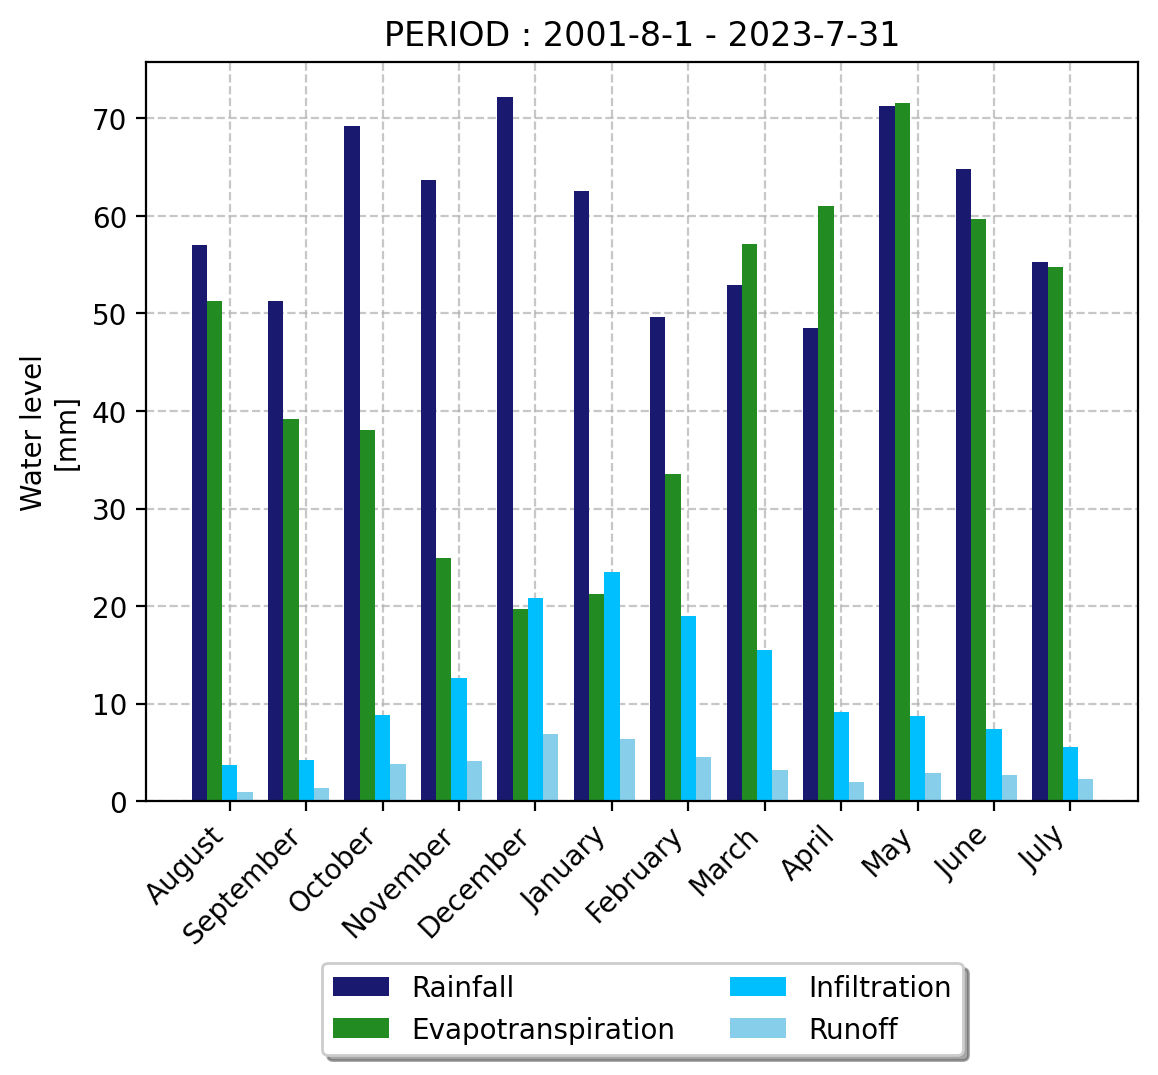
\includegraphics[width=0.55\linewidth]{
        3_features/fig/BUDGET_2001-8-12023-7-31Pluriannual_Sum.png
    }
    \caption{Exemple de rendu graphique du bilan hydrologique mensuel
    pluriannuel simulé}
    \label{fig-budget-barplot}
\end{figure*}

\newpage
\section{\script{Hydological Regime}: Visualisation des régimes hydrologiques}
\label{sec-regime-hydro}

Les régimes hydrologiques de l'hydrosystème simulés sont construits à partir de la
boite de dialogue \gui{Hydrological Regime} (cf. Figure
\ref{fig-dialogHydroRegime}). Les régimes hydrologiques sont calculés sur la
période renseignée dans les zones de saisie \gui{Start} et \gui{end}. La variable
analysée est à préciser dans le menu déroulant \gui{Hydrological variable to plot}. Le type de rendu est choisi par l'utilisateur en cochant les case \gui{static plots (PNG)} pour un rendu des graphiques sous la forme d'image unique pour chaque point de mesure, \gui{static plots (PDF)} pour un rendu sous forme pdf compilant les régimes hydrologiques de tous les points de mesure et enfin \gui{interractives plots} pour un rendu dans le navigateur par défaut sous la forme de graphique interactifs (\ref{fig-output-regime-hydrologique}. Une boite de dialogue avertit l'utilisateur de la fin de l'exécution du module de calcul.\\

\begin{figure}[h]
    \centering
    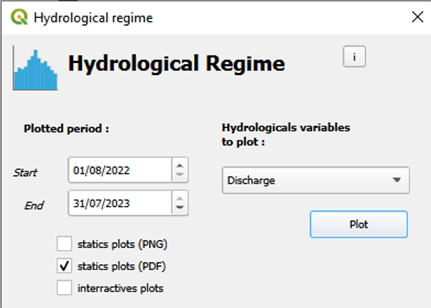
\includegraphics[width=0.5\linewidth]{
        3_features/fig/DialogHydrologicalREgime.png
    }
    \caption{Boite de dialogue \gui{Hydrological Regime} permettant le calcul des
    régimes hydrologiques mensuels pluriannuels.}
    \label{fig-dialogHydroRegime}
\end{figure}


\begin{figure*}[htb]
    \centering
    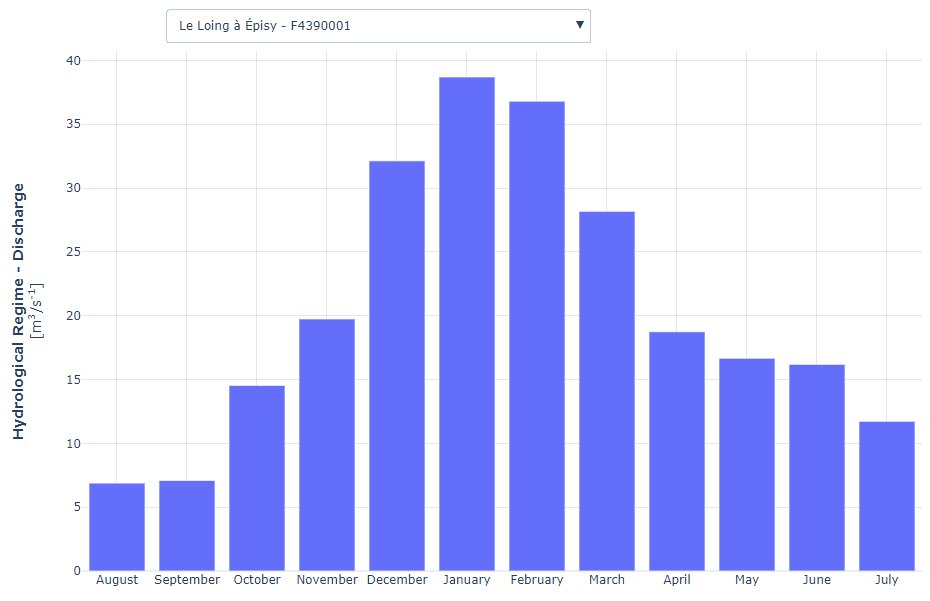
\includegraphics[width=0.5\linewidth]{
        3_features/fig/Output_regime_hydrologique.png
    }
    \caption{Exemple de rendu graphique du régime hydrologique mensuel
    pluriannuel simulé}
    \label{fig-output-regime-hydrologique}
\end{figure*}

\newpage
\section{\script{Extract Data from a sub area}: Extraction des resultats dans un polygon}
\label{sec-extract-area}

La boîte de dialogue \gui{Extract Data from a Sub Area} permet d’extraire les résultats des simulations sur une zone définie. Cette zone peut être spécifiée soit comme un polygone provenant d’un QGSVectorLayer chargé dans le projet, soit comme un shapefile importé depuis un répertoire.

Les résultats sont enregistrés sous forme de fichiers CSV (analyses) et de fichiers NumPy contenant les données de la zone extraite. Ces fichiers permettent de relancer les analyses à partir de la configuration créée.

\subsection*{Variables d’extraction}
À partir de la boîte de dialogue, il est possible de choisir les variables suivantes pour l’extraction :
\begin{itemize}
    \item Nom du nouveau fichier d’extraction (également utilisé comme nom du dossier créé dans \texttt{PostProcessing/DATA\_EXTRACTED/})
    \item Polygone d’extraction : soit un shapefile (à tester), soit un QGSVectorLayer présent dans le projet
    \item Période d’extraction
    \item Résolution de l’extraction pour le module WATBAL (à confirmer si nécessaire)
\end{itemize}

Les sorties dépendent des cases cochées dans la colonne de droite.

\subsection*{Sorties -- Bilan hydrologique (WATBAL)}
\gui{Rainfall} \gui{Real EvapoTranspiration (ET)} \gui{Infiltration} \gui{Runoff} \gui{Potential EvapoTranspiration (ET)}

Ces options fournissent les résultats du bilan hydrologique (WATBAL). Les données sont sauvegardées dans un fichier CSV sous forme agrégée sur toute la période de simulation, avec une valeur par cellule.

\subsection*{Sorties -- Régime hydrologique (HYD)}
\gui{Surface flow}

\begin{itemize}
    \item Tous les biefs en contact avec la bordure du polygone sont définis comme points d’extraction.
    \item Le fichier CSV contient les données journalières de débit et de hauteur d’eau pour chaque point situé sur la limite du polygone.
    \item La convention de signe pour le débit est la suivante : positif en entrée, négatif en sortie.
    \item Des fichiers NumPy sont également générés, permettant de relancer et d’approfondir les analyses sur ces données.
\end{itemize}

\subsection*{Sorties -- Aquifère}
\gui{Subsurface flow}

\begin{itemize}
    \item Pour chaque couche de l’aquifère, les limites du polygone sont définies avec la résolution propre à la couche.
    \item Un fichier CSV est généré pour chaque couche.
    \item Les flux sont fournis à une échelle journalière pour chaque face située à la limite de l’aquifère.
    \item Les faces sont nommées selon la convention : \texttt{nCell(ID\_ABS)\_direction\_unité}, par exemple : \texttt{3323\_west\_m3d}.
\end{itemize}

\subsection*{Organisation des outputs}

Pour chaque extraction, des fichiers de résultats et des couches sont produits.

Les fichiers sont sauvegardés dans le répertoire de sortie défini dans les paramètres de l’analyse principale :
\texttt{PostProcessing/DATA\_EXTRACTED/<Nom\_Extraction>}

On y trouve :
\begin{itemize}
    \item \textbf{CONFIG/} : fichiers de configuration permettant de relancer les simulations
    \item \textbf{OUTPUT/} : fichiers CSV contenant les résultats
    \item \textbf{TEMP/} : fichiers NumPy utilisés pour relancer les analyses
\end{itemize}

Dans QGIS, des maillages (\textit{mesh}) sont également générés pour chaque compartiment extrait.
    \chapter{Description du code}
\label{chap-description-src}

\renewcommand{\headrulewidth}{0.3pt}
\fancyhead[LE]{\thepage} \fancyhead[RE]{\nouppercase{\textbf{\leftmark}}}
\fancyhead[RO]{\thepage} \fancyhead[LO]{\nouppercase{\textbf{\rightmark}}}
\fancyfoot[L,C,R]{}

\setlength{\parindent}{0.35cm}

\minitoc

% ================================================================

Le plug-in \cwv~est une classe Python à part entière (\gui{cawaqs\_viz.py}).
Cette classe gère notamment les fonctions de chargement du plug-in dans l'interface
QGIS et fait le lien avec les boîtes de dialogue de l'interface. Le plug-in \cwv~est
structuré autour de quatre classes principales (cf. Fig.
\ref{fig-structure_cawaqs_viz}) :
\begin{itemize}
    \item \gui{Compartement} et \gui{Manage} (\textit{backend}) sont des classes
        de gestion des objets attachées à la structure du modèle \cawaqs~. Elles
        regroupent l'ensemble des fonctionnalités d'analyse des résultats de
        simulation ;

    \item \gui{ExploreData} (\textit{passerelle}) est une classe de gestion des objets
        du \textit{backend} et permet de naviguer au sein des objets initialisés
        au cours de l'utilisation du plug-in ;

    \item \gui{Dialog} (\textit{frontend}) est la classe mère de toutes les boîtes
        de dialogue du plug-in. Chaque action de calcul et d'analyse des
        résultats de simulation est lancée depuis ces boîtes de dialogue.
\end{itemize}

Les utilitaires additionnels sont contenus dans le répertoire \gui{./tools}. Ils
incluent notamment des fonctions de gestion et de traitement des objets QGIS (fonction
de création de couche, modification de table attributaire, ajouts d'entités dans
une table attributaire, actualisation de table par exemple, etc.), ainsi que les
fonctions de calcul des critères statistiques appelées dans les méthodes de
classe de \gui{Manage}.\\

Les boîtes de dialogue sont créées et modifiées avec l'outil \gui{QT Designer},
outil livré à l'installation de QGIS. Tous les objets inhérents aux boîtes de dialogue
sont inclus \textit{via} cette application. \gui{QT Designer} crée le fichier d'extension
\script{.ui} appelé par la classe de l'objet. D'une façon générale, ce fichier gère
l'apparence de la boîte de dialogue et de ses objets graphiques. Chaque boîte de
dialogue est donc une classe qui appelle son fichier \script{.ui} à l'initialisation
de la classe. \\

Les fonctionnalités d'analyse sont actionnées par un bouton d'action spécifique ou
simplement à l'exécution de la boîte de dialogue \textit{via} son bouton d'exécution
\gui{OK}. Chaque bouton d'action est rattaché à une méthode de classe de sa
boîte de dialogue. Ces méthodes appellent la classe \gui{ExploreData} pour
naviguer dans les objets initialisés et la classe \gui{Manage} si un traitement de
données est nécessaire. Les fonctionnalités inhérentes à l'utilisation des
objets QGIS (ex : affichage de rendus cartographiques, actualisation de couche, etc.)
sont directement gérées par les méthodes de classe des boîtes de dialogue qui peuvent
parfois faire appel aux utilitaires additionnels (\gui{tools}) si les actions
sont partagées entre plusieurs boîtes de dialogue.

\begin{landscape}
    \begin{figure*}
        \centering
        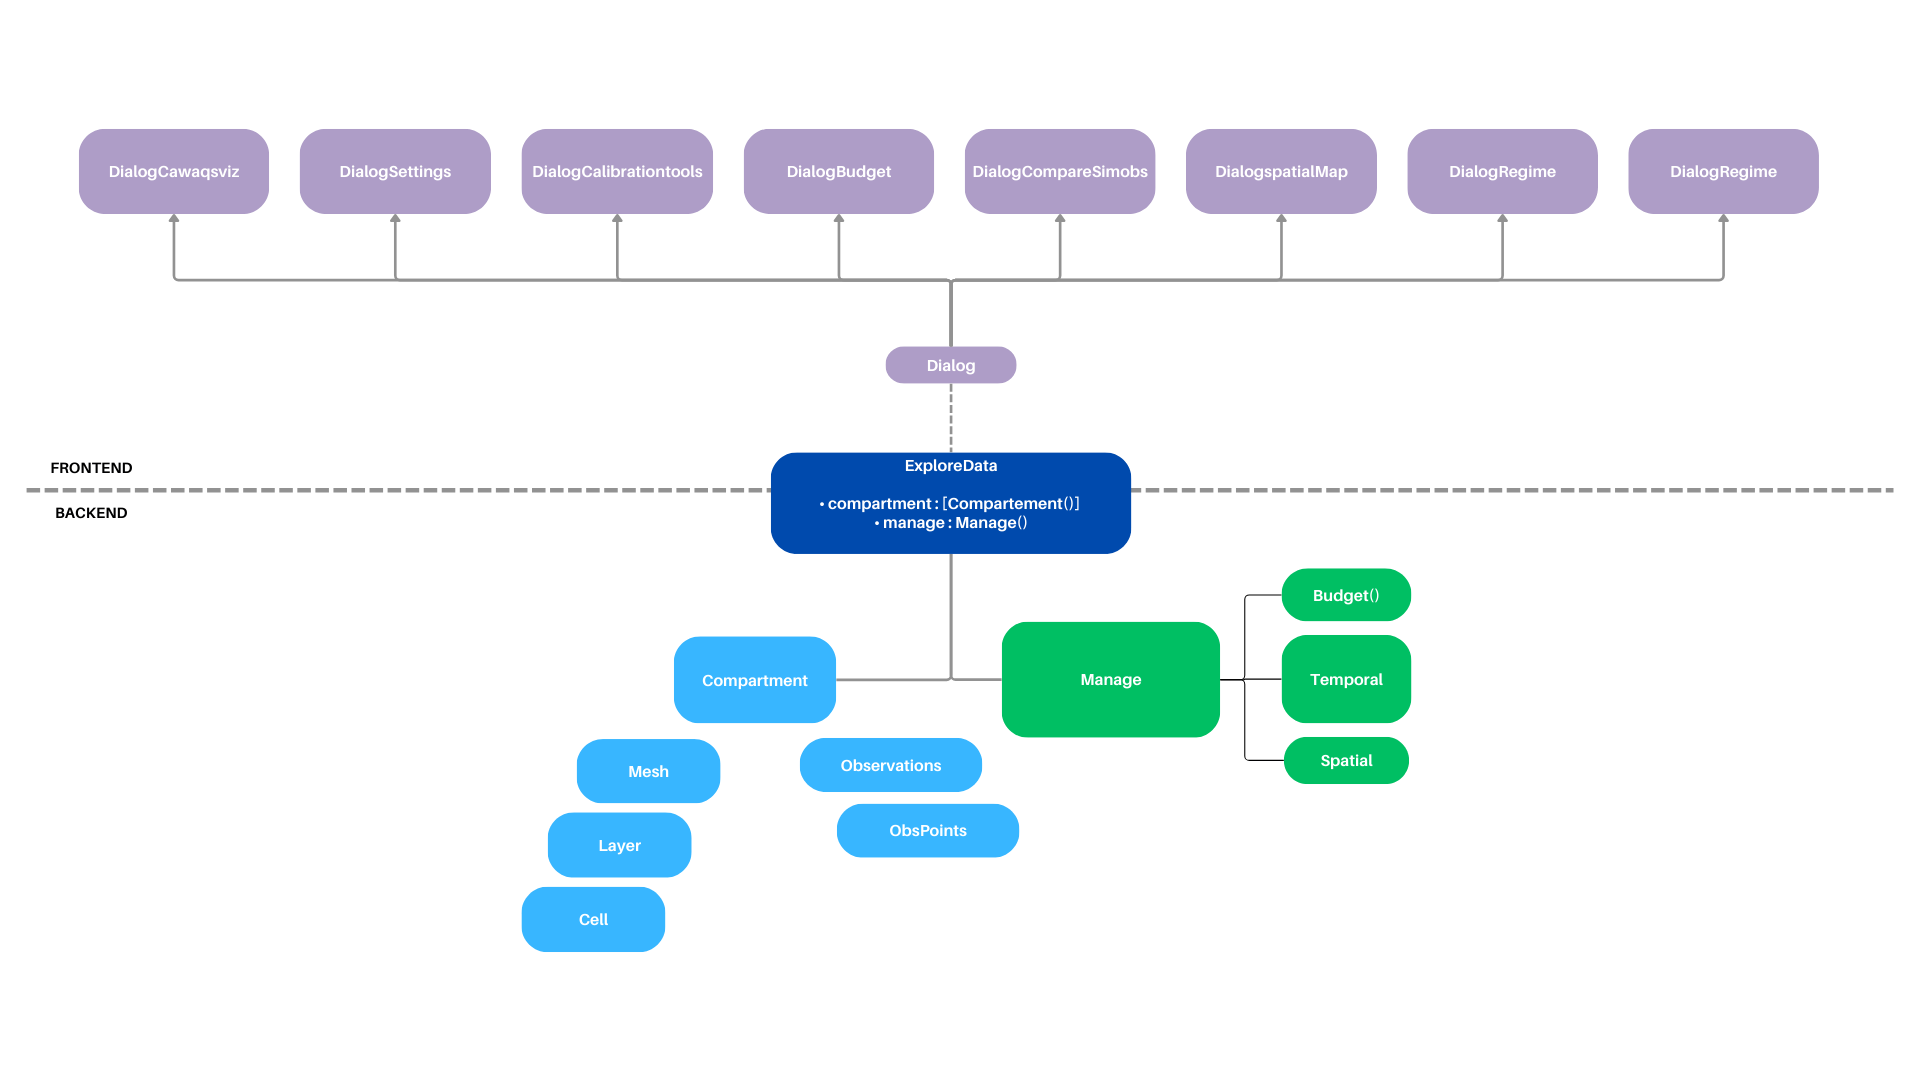
\includegraphics[width=1\linewidth]{
            4_application_scripts/fig/schema_conceptuel_cwv.png
        }
        \caption{Structure du code source du plug-in \cwv.}
        \label{fig-structure_cawaqs_viz}
    \end{figure*}
\end{landscape}

% \section{Détail du back-end}\label{sec-backend}

% ...

% \section{Détail du front-end}\label{sec-frontend}

% ...

% \section{Détail de la passerelle}\label{sec-passerelle}

% ...
    \chapter{Consignes aux développeurs}

\section{Architecture du code}
Le code s'organise autour d'un backend et d'un frontend constitué autour des classes des boites de dialogues. Le backend embarque les fonctionnalité de traitement des simulations (lecture des fichiers, traitements hydrologique, etc), ainsi que les classes des éléments de maillage de \cws. Des classes "paserelles" de configuration de l'application depuis l'instance de QGIS et de navigation dans les données de simulations et les éléments de maillage lié la backend et le fondend. 

\subsection{Le backend} 
Embarquant les classes (\script{Mesh}, \script{Layer},  \script{Cell}) constituant le maillage \cws~ à partir de couches \script{shapefiles} présentent dans le projet QGIS, le backend permet également le traitement et l'analyse hydrologique des simulations, géré par la classe \script{Manage}. La classe de traitement \script{Manage} permet de le traitement temporel (\script{Temporal})et  spatial \script{Spatial} des simulations ainsi que le calcul des bilans hydrologiques et hydrogéologiques (\script{Budget}). La classe \script{Compartment} construit répertorie les éléments de maillages construit avec \script{Mesh} qui elle-même appelle à la classe \script{Mesh} qui construit les couches du compartiment (une seule couche par compartiment excepté pour le compartiment aquifère). \script{Compartiment} intègre également les chemins de répertoire de simulation des variables hydrologiques simulé pour le dit compartiment et le répertoire des variables observés. Il embarque également en attribut la classe \script{Observation} intégrant les \script{ObservationPoint} quand ils sont précisés, et la classe \script{Extraction} intégrant les \script{ExtractionPoints} quand ils existents.\\
Enfin, le fichier \script{parameters.py} intègre toutes les variables de paramétrage de la classe \script{Manage} inhérante à la structure d'écriture de \cws à savoir les champs écrits dans les fichiers binaires, les formats d'écriture ainsi qu'à la structure du code de \cws, à savoir les noms des compartiments, leur index, les noms des sous répertoire de sortie écrit par \cws pendant le simulation, les strucutres des fichiers \script{corresp\_file} écrit par la plateforme \cws en de simulation pour chaque compartiment dont les processus sont simulés. La distinction de ces variables permets de modifier les paramètres de l'application sans modifier toutes les variables dans les différentes classes du code. 

\subsection{La frontend}
Le frontend est constitué des classes de boites de dialogue de l'application associé à leurs fichiers \script{.ui} qui définie les objets \script{Qt} présent dans la boite de dialogue (champs, liste, texte, etc.). Ces boites de dialogues sont créer à partie de l'application \script{Qt Designer}\footnote{téléchargable depuis le lien \href{https://build-system.fman.io/qt-designer-download}{https://build-system.fman.io/qt-designer-download}}, application embarquée avec QGIS. La section \ref{sec_QtDesigner} précise comment utiliser l'application de designe des boite de dialogue et comment elle s'intègre dans l'application \cwv. Le frontend de l'application gère directement l'appelle des fonctions du backend et le traitement des données gérées par \script{ExploreData} en fonction des demandes de l'utilisateur. Le lancement d'un processus peut s’exécuter directement à la validation de la boite de dialogue via le bouton \script{ok}, à la fermeture de la boite de dialogue, où par un bouton de commande autre dans la boite de dialogue (exemple : la boite de dialogue \script{SpatialMap} contient autant de bouton que de variables hydrologiques pouvant être spatialisé par l'application \cws). 

\subsection{Les passerelles}
Les classes passerelles que sont \script{ExploreData} et \script{Config}, sont pour la première, une classe de naviguation dans les données de simulation et de maillage d'une simulation \cws, pour la seconde, une classe de configuration de l'application \cws depuis une configuration de projet QGIS. La classe configuration écrit au format \script{json} la configuration géométrique du projet QGIS (\script{config\_geometrie.json}) et  la configuration du projet de simulation (\script{config\_projet}) embarquant les informations nécessaires au traitement des simulations \cws~, à savoir les périodes de simulations, le répertoire de sortie des simulations, les répertoires des observations quand elles existent, la configuration géométrique du projet QGIS, le régime de simulation et les compartiments dont les processus hydrologiques sont simulés. Cette classe permet ensuite de configurer la classe \script{ExploreData} qui fait appelle au backend de l'application en construisant les compartiments de la simulation. 

\begin{figure}[H]
    \centering
    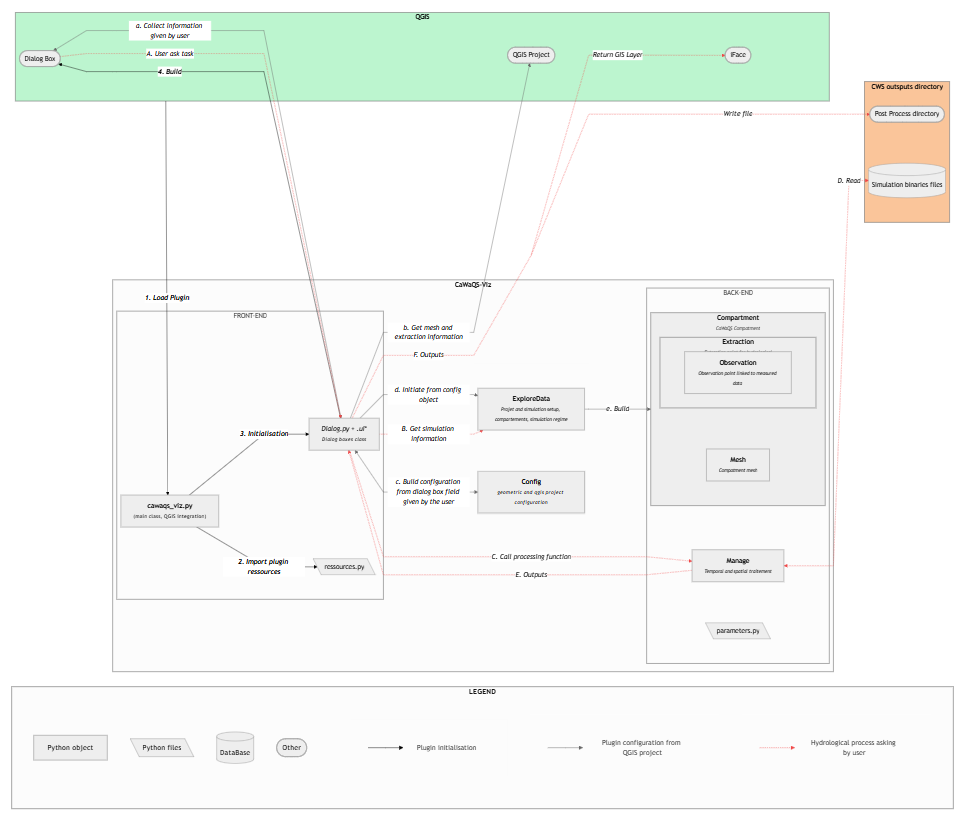
\includegraphics[width=1\linewidth]{5_develloppeur/fig/schema_cwv.png}
    \caption{Schéma fonctionnel de l'application \cwv}
    \label{fig_fonctionnement_cwv}
\end{figure}

\section{Mise à jour de la version} 

La version du plugin est renseignée dans le fichier \script{metadata.txt} contenu dans l'extrait de code \ref{code_metadata}.
\begin{lstlisting}[language=json, caption={Informations obligatoires à renseginer dans le fichier \script{metadata.txt}}, label={code_metadata}]
[general]
name=CaWaQS-Viz
qgisMinimumVersion=3.0
description=Description
version=0.1.16
author=Lise-Marie GIROD (Mines Paris - PSL), Nicolas Flipo (Mines Paris - PSL)
email=lise-marie.girod@minesparis.psl.eu

about=Python QGIS-based vizualization software for CaWaQS3.x

repository=https://gitlab.com/gviz/cawaqsviz
\end{lstlisting}

\section{Documentation du code} 

La documentation du code est publiée sur le lien suivant via gitlab Pages au lien suivant : \href{https://cawaqsviz-gviz-adf347ff6d9d45c174db091497a2dfc0f14305cdb4ed9070.gitlab.io/}{https://cawaqsviz-gviz-adf347ff6d9d45c174db091497a2dfc0f14305cdb4ed9070.gitlab.io/}. L'alimentation de la documentation est assurée par la tenue des docstrings dans les modules de l'application, selon le formatage présenté en exemple. 


\begin{lstlisting}[language=Python, caption={Formatage de la docstring pour intégration automatique dans la documentation du code}, label={code_format_docstrings}]
class Exemple:
    """
    Resume des fonctionnalites de la classe.
    """

    def __init__(self, arg1):
        """
        Methode constructeur.

        :param arg1: descriptif du parametre
        :type arg1: str
        """
        self.arg1 = arg1

    def do_something(self, arg1: list) -> str:
        """
        Descriptif de la fonction.

        :param arg1: descriptif du parametre
        :type arg1: list
        :return: descriptif de ce que la fonction retourne
        :rtype: str
        """
        return ", ".join(map(str, arg1))
\end{lstlisting}
\vspace{1em}
La compilation est opérée par \script{Sphinx}\footnote{dont la documentation est accecible via \href{https://www.sphinx-doc.org/en/master/}{https://www.sphinx-doc.org/en/master/}}. Le répertoire \script{docs/sources} contient les fichiers de configuration (\script{Conf.py}), ainsi que le contenu de la documentation. 
Dans le cas de l'intégration de nouvelles dans le plugin, leur intégration dans l'index (\script{index.rst}) est nécessaire pour que la docstring du code apparaisse dans le page de documentation. Cet index est intègre 3 fichiers  : \script{frontend.rst}, \script{interface.rst}, \script{backend.rst} qui contiennent les classes à documentés. L'intégration d'un nouveau module dans l'application nécessite d'être ajouté dans ces fichiers sous la forme de l'extrait de code \ref{code_format_rst}. Les mises à jour des fichiers sources de la documentation doivent être commité et synchronisé avec les dépôts. 

\begin{lstlisting}[language=Python,caption={Formatage de la docstring pour intégration automatique dans la documentation du code}, label={code_format_rst}]
Module
------

.. automodule:: cawaqsviz.Module
   :members:
   :show-inheritance:
   :undoc-members:
\end{lstlisting}

\vspace{1em}

Finalement à chaque nouveau commit dans les branche \script{Main} ou 
\script{Beta}, la documentation est compilée selon le contenu du répertoire \script{docs/source} du dépôt.

\begin{lstlisting}
image: python:3.9

stages:
  - build
  - deploy

before_script:
  - pip install -U pip
  - pip install -r requirements.txt

build-docs:
  stage: build
  script:
    - sphinx-build -b html docs/source public
  artifacts:
    paths:
      - public

pages:
  stage: deploy
  script:
    - echo "Pages deployed"
  artifacts:
    paths:
      - public
  only:
    - main  
    - beta

\end{lstlisting}

\newpage
\section{Outils de débogage}
\subsection{Le plugin \script{Plugin Reloader}}

Cet utilitaire permet de recharger un plugin après une modification de son code. Ainsi il n'est pas nécessaire de recharger QGIS à chaque modification de code. 

Le plugin est installable depuis le gestionnaire d'extention de \script{QGIS}.

\begin{figure}[H]
    \centering
    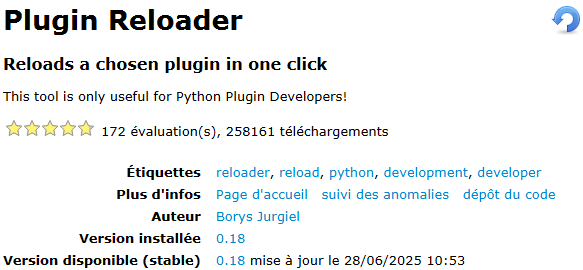
\includegraphics[width=0.75\linewidth]{5_develloppeur/fig/plugin_reloader.png}
    \caption{Fiche descriptive de \script{Plugin Reloader}}
    \label{fig_plugin_reloader}
\end{figure}

\subsection{Le plugin QGIS \script{First Aid}}

Le plugin \script{First Aid} permet d'investiger les erreurs survenant à l'exution du plugin 


\newpage
\subsection{VS-Code}
Le plugin \script{debugvs} permet de connecté une instance de débogage \script{VS-Code} à l’exécution du plugin depuis QGIS. Cette configuration de debugage permet d'utiliser toute les fonctionnalités de VS Code durant le debugague (breakpoint, espion, pile d'appels...).  La mise en place de cette configuration de debugage est réalisée de la manière suivante : 
\begin{enumerate}
    \item installer \script{debugpy} avec la commande \script{!pip install debugpy} depuis l'invité de commande Python de QGIS ;
    \item \sloppy si le répertoire de développement du plugin ne se situe pas dans le répertoire \texttt{C://Users/$USER$/AppData//QGIS/QGIS3/profiles/default/python}, créer un lien symbolique dans ce repertoire pointant vers le répertoire de développement.  
    \item installer le plugin \script{debugvs} en téléchargeant son script depuis le dépôt Gitlab \url{https://github.com/lmotta/debug_vs} et activer le plugin en important le dossier \script{.zip} dans \script{QGIS} (\cffig \ref{fig_debugvs}) ; 
    \begin{figure}[H]
        \centering
        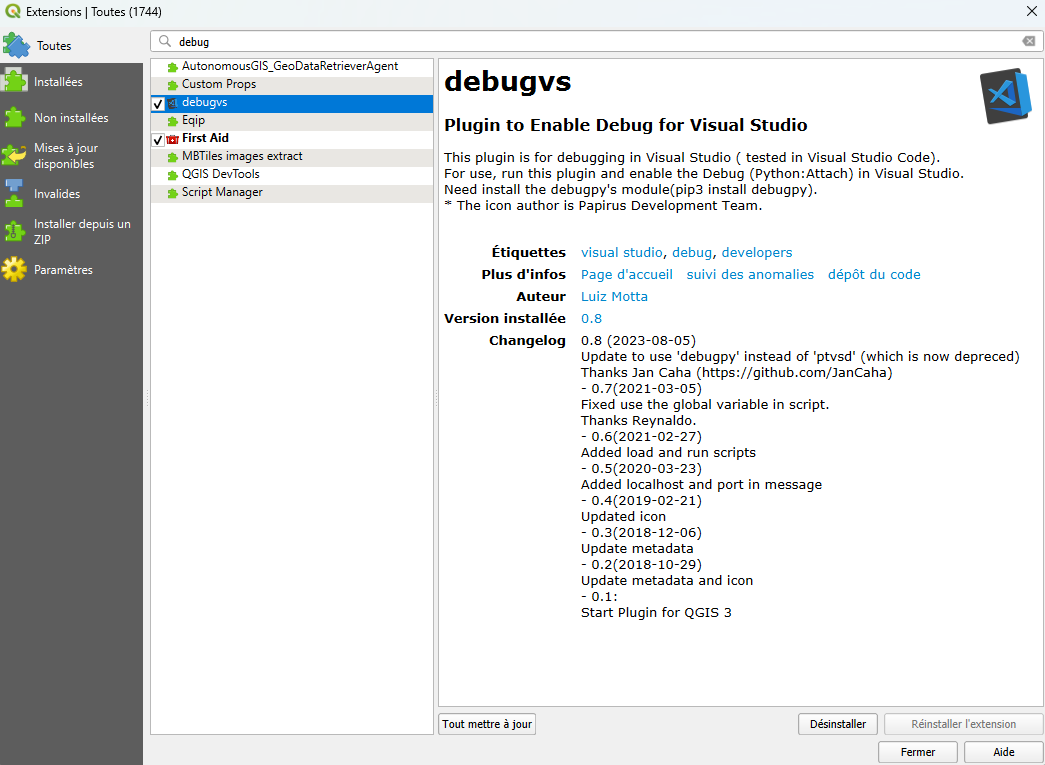
\includegraphics[width=0.6\linewidth]{5_develloppeur/fig/debugvs.png}
        \caption{Pluging \script{debugvs}}
        \label{fig_debugvs}
    \end{figure}
    \item configurer VS Code pour se connecter à QGIS durant une session de debuggage : 
    \begin{enumerate}
        \item dans le répertoire de développement du CaWaQS-Viz, créer un sous-répertoire \script{.vscode} (ajouter ce répertoire au fichier \script{.gitignore}) ; 
        \item créer un fichier \script{settings.json} dans le sous-répertoire \script{.vscode} et copier du contenu du code \ref{code_settings_vscode}.Modifier éventuellement les chemins d'accès au répertoire pour qu'ils correspondent à votre installation de QGIS et de Python et à votre système opératif. Celui-là, c'est pour Windows.
        \begin{lstlisting}[language=JSON, caption={Fichier de configuration du workspace. Ce fichier définit la configuration du workspace Visual Studio Code pour le développement du plugin QGIS. Il permet d’adapter l’environnement Python de VS Code à celui utilisé par QGIS (installé via OSGeo4W).}, label=code_settings_vscode]
        {   
            
            "workbench.colorCustomizations": {
                "titleBar.activeBackground": "#006823",
                "editor.background": "#000000"
            },
            
            "python.linting.pylintEnabled": true,
            "python.jediEnabled": true,
        
            
            "python.pythonPath": "C:/OSGeo4W64/bin/python-qgis.bat",
        
        
            "python.linting.pylintArgs": [
                "--extension-pkg-whitelist=PyQt5,qgis,db_manager",
                "--disable=all",
                "--enable=F,E,unreachable,duplicate-key,unnecessary-semicolon,global-variable-not-assigned,unused-variable,binary-op-exception,bad-format-string,anomalous-backslash-in-string,bad-open-mode"
            ],
        
           
            "terminal.integrated.env.windows": {
                
                "PATH": "C:\\OSGeo4W\\apps\\qgis\\bin;C:\\OSGeo4W\\apps\\Python312;C:\\OSGeo4W\\apps\\Python312\\Scripts;C:\\OSGeo4W\\apps\\Qt5\\bin;C:\\OSGeo4W\\apps\\Python312\\Scripts;C:\\OSGeo4W\\bin;C:\\Windows\\System32;C:\\Windows;C:\\Windows\\system32\\WBem;C:\\OSGeo4W\\apps\\Python312\\lib\\site-packages\\pywin32_system32;C:\\OSGeo4W\\apps\\Python312\\lib\\site-packages\\numpy\\.libs",
                
                "PYTHONHOME": "C:\\OSGeo4W\\apps\\Python312",
                "PYTHONPATH": "C:\\OSGeo4W\\apps\\qgis\\python;%PYTHONPATH%",
                
                "GDAL_DATA": "C:\\OSGeo4W\\share\\gdal",
                "GDAL_DRIVER_PATH": "C:\\OSGeo4W\\bin\\gdalplugins",
                "GDAL_FILENAME_IS_UTF8": "YES",
                
                "GEOTIFF_CSV": "C:\\OSGeo4W\\share\\epsg_csv",
                
                "O4W_QT_BINARIES": "C:/OSGeo4W/apps/Qt5/bin",
                "O4W_QT_DOC": "C:/OSGeo4W/apps/Qt5/doc",
                "O4W_QT_HEADERS": "C:/OSGeo4W/apps/Qt5/include",
                "O4W_QT_LIBRARIES": "C:/OSGeo4W/apps/Qt5/lib",
                "O4W_QT_PLUGINS": "C:/OSGeo4W/apps/Qt5/plugins",
                "O4W_QT_PREFIX": "C:/OSGeo4W/apps/Qt5",
                "O4W_QT_TRANSLATIONS": "C:/OSGeo4W/apps/Qt5/translations",
                "QT_PLUGIN_PATH": "C:\\OSGeo4W\\apps\\qgis\\qtplugins;C:\\OSGeo4W\\apps\\Qt5\\plugins",
                
                "QGIS_PREFIX_PATH": "C:/OSGeo4W/apps/qgis",
                
                "VSI_CACHE": "TRUE",
                "VSI_CACHE_SIZE": "1000000"
            },
            "python.languageServer": "Jedi", 
        }
\end{lstlisting} 
        \item créer un fichier \script{launch.json} dans le sous répertoire \script{.vscode}, copier le contenu du code \ref{code_launch_vscode}, modifier les chemin d'accès \script{localRoot} et \script{remoteRoot} pour correspondre à la configuration de votre espace de travail.
        
        \begin{lstlisting}[language=JSON, caption={Fichier de configuration du debugger VS-Code. Dans cette configuration, la section "connect" indique l’adresse et le port sur lesquels QGIS expose la session de débogage (ici localhost:5678). Le bloc "pathMappings" établit la correspondance entre les chemins locaux du projet ouvert dans VS Code (localRoot) et les chemins utilisés par QGIS pour exécuter le plugin (remoteRoot). Cette correspondance est essentielle pour que les breakpoints placés dans VS Code soient correctement associés aux fichiers réellement exécutés par QGIS.}, label = code_launch_vscode]
{
    "version": "0.2.0",
    "configurations": [
        {
            "name": "Attach QGIS Debug",
            "type": "python",
            "request": "attach",
            "connect": {
                "host": "localhost",
                "port": 5678
            },
            "pathMappings": [
                {
                    "localRoot": "C:\\Program Files\\$QGIS$\\apps\\qgis-ltr\\python\\plugins\\cawaqsviz",
                    "remoteRoot": "C:\\Users\\$USER$\\AppData\\Roaming\\QGIS\\QGIS3\\profiles\\default\\python\\cawaqsviz"
                }
            ],
            "justMyCode": false
        }
    ]
}


\end{lstlisting}
        \end{enumerate}
    \item Établir la connexion QGIS/VS-Code
    \begin{enumerate}
        \item autoriser la connexion du debugueur à QGIS par le plugin \script{debugvs} (\cffig \ref{fig_enable_vscode_qgis}) ;
        \begin{figure}[H] 
            \centering
            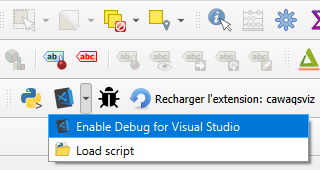
\includegraphics[width=0.40\linewidth]{5_develloppeur/fig/launch_debug_vs.png}
            \caption{Établissement d'une connexion QGIS/VS-Code depuis le plugin \script{debugvs}}
            \label{fig_enable_vscode_qgis}
        \end{figure}
        \item lancer la session de debugage VS-Code (\cffig \ref{fig_debug_VS_CODE}).
        \begin{figure}[H]
            \centering
            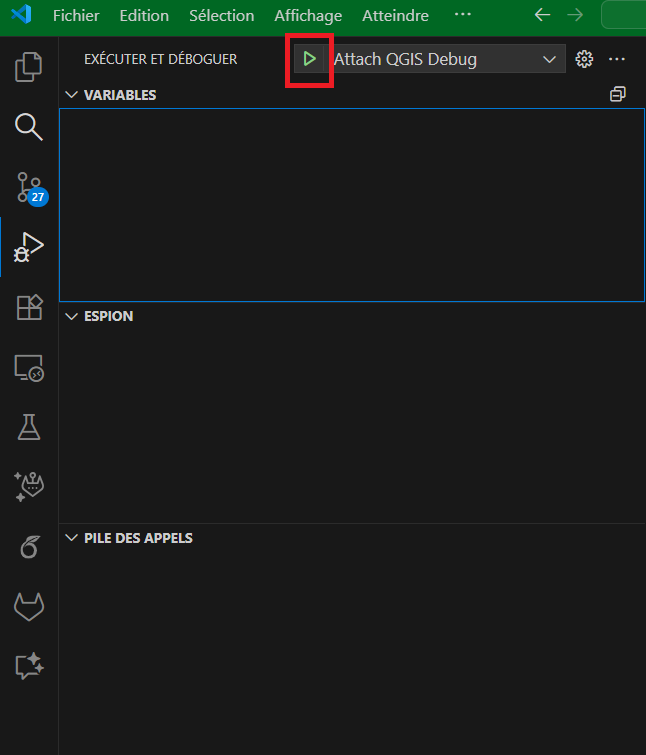
\includegraphics[width=0.5\linewidth]{5_develloppeur/fig/debug_vs_code.png}
            \caption{Lancement d'une session de debuguage depuis VS-Code}
            \label{fig_debug_VS_CODE}
        \end{figure}
    \end{enumerate}
\end{enumerate} 

La connexion entre le debbuger et QGIS est interrompue depuis VS-Code en cliquant sur \script{"Disconnected"} dans la barre d'outil de debuggage (\cffig \ref{fig_barre_outil_debbug}) 

\begin{figure}[H]
    \centering
    
\includegraphics[width=0.35\linewidth]{5_develloppeur/fig/disconnect-debugger.png}
    \caption{Barre d'outil du debugger VS-Code}
    \label{fig_barre_outil_debbug}
\end{figure}






\newpage
\section{Création des boites de dialogue avec \script{Qt Designer}} 
\ref{sec_QtDesigner}
L'application \script{Qt Designer}, livrée à l'installation de QGIS (installation avec OSGEO), est un outil de création de boite de dialogue sous la forme de fichier .ui. Dans l'application \cwv, toutes les boites de dialogues ont leur propre fichier \script{.py} auquel le fichier \script{.ui}, du même nom, est associé à la classe python de la boite de dialogue. 

\begin{lstlisting}[language = Python, label = code_init_from_ui, caption = Initialisation de la boite de dialogue "Compare SIM/OBS" depuis un fichier .ui]
# This loads your .ui file so that PyQt can populate your plugin with the elements from Qt Designer
FORM_CLASS, _ = uic.loadUiType(
    os.path.join(os.path.dirname(__file__), "DialogComparesimobs.ui")
)


class DialogComparesimobs(Dialog, FORM_CLASS):
    def __init__(self, iface:QgisInterface, log_file_path:str, parent=None):
        """Constructor Method

        :param iface: Qgis Interface
        :type iface: QgisInterface
        :param logFilePath: Path of the cawaqs-viz log file, defaults to None
        :type logFilePath: str, optional
        :param parent: Parent class, defaults to None
        :type parent: _type_, optional
        """
        super(DialogComparesimobs, self).__init__(parent)
        self.setupUi(self)
        self.iface = iface
        self.logFilePath = log_file_path
        self.simData = False
\end{lstlisting}



    \phantomsection

\renewcommand{\headrulewidth}{0.3pt} 
\fancyhead[LE]{\thepage} 
\fancyhead[RE]{\nouppercase{\textbf{Bibliographie}}}
\fancyhead[RO]{\thepage} 
\fancyhead[LO]{\nouppercase{\textbf{Bibliographie}}}
\fancyfoot[L,C,R]{}

\setlength{\parindent}{0.35cm} 

\bibliographystyle{apalike-fr}
\addcontentsline{toc}{chapter}{\bibname}
\bibliography{references}
\end{document}